% Options for packages loaded elsewhere
\PassOptionsToPackage{unicode}{hyperref}
\PassOptionsToPackage{hyphens}{url}
%
\documentclass[
]{article}
\usepackage{amsmath,amssymb}
\usepackage{lmodern}
\usepackage{iftex}
\ifPDFTeX
  \usepackage[T1]{fontenc}
  \usepackage[utf8]{inputenc}
  \usepackage{textcomp} % provide euro and other symbols
\else % if luatex or xetex
  \usepackage{unicode-math}
  \defaultfontfeatures{Scale=MatchLowercase}
  \defaultfontfeatures[\rmfamily]{Ligatures=TeX,Scale=1}
\fi
% Use upquote if available, for straight quotes in verbatim environments
\IfFileExists{upquote.sty}{\usepackage{upquote}}{}
\IfFileExists{microtype.sty}{% use microtype if available
  \usepackage[]{microtype}
  \UseMicrotypeSet[protrusion]{basicmath} % disable protrusion for tt fonts
}{}
\makeatletter
\@ifundefined{KOMAClassName}{% if non-KOMA class
  \IfFileExists{parskip.sty}{%
    \usepackage{parskip}
  }{% else
    \setlength{\parindent}{0pt}
    \setlength{\parskip}{6pt plus 2pt minus 1pt}}
}{% if KOMA class
  \KOMAoptions{parskip=half}}
\makeatother
\usepackage{xcolor}
\usepackage[margin=1in]{geometry}
\usepackage{color}
\usepackage{fancyvrb}
\newcommand{\VerbBar}{|}
\newcommand{\VERB}{\Verb[commandchars=\\\{\}]}
\DefineVerbatimEnvironment{Highlighting}{Verbatim}{commandchars=\\\{\}}
% Add ',fontsize=\small' for more characters per line
\usepackage{framed}
\definecolor{shadecolor}{RGB}{248,248,248}
\newenvironment{Shaded}{\begin{snugshade}}{\end{snugshade}}
\newcommand{\AlertTok}[1]{\textcolor[rgb]{0.94,0.16,0.16}{#1}}
\newcommand{\AnnotationTok}[1]{\textcolor[rgb]{0.56,0.35,0.01}{\textbf{\textit{#1}}}}
\newcommand{\AttributeTok}[1]{\textcolor[rgb]{0.77,0.63,0.00}{#1}}
\newcommand{\BaseNTok}[1]{\textcolor[rgb]{0.00,0.00,0.81}{#1}}
\newcommand{\BuiltInTok}[1]{#1}
\newcommand{\CharTok}[1]{\textcolor[rgb]{0.31,0.60,0.02}{#1}}
\newcommand{\CommentTok}[1]{\textcolor[rgb]{0.56,0.35,0.01}{\textit{#1}}}
\newcommand{\CommentVarTok}[1]{\textcolor[rgb]{0.56,0.35,0.01}{\textbf{\textit{#1}}}}
\newcommand{\ConstantTok}[1]{\textcolor[rgb]{0.00,0.00,0.00}{#1}}
\newcommand{\ControlFlowTok}[1]{\textcolor[rgb]{0.13,0.29,0.53}{\textbf{#1}}}
\newcommand{\DataTypeTok}[1]{\textcolor[rgb]{0.13,0.29,0.53}{#1}}
\newcommand{\DecValTok}[1]{\textcolor[rgb]{0.00,0.00,0.81}{#1}}
\newcommand{\DocumentationTok}[1]{\textcolor[rgb]{0.56,0.35,0.01}{\textbf{\textit{#1}}}}
\newcommand{\ErrorTok}[1]{\textcolor[rgb]{0.64,0.00,0.00}{\textbf{#1}}}
\newcommand{\ExtensionTok}[1]{#1}
\newcommand{\FloatTok}[1]{\textcolor[rgb]{0.00,0.00,0.81}{#1}}
\newcommand{\FunctionTok}[1]{\textcolor[rgb]{0.00,0.00,0.00}{#1}}
\newcommand{\ImportTok}[1]{#1}
\newcommand{\InformationTok}[1]{\textcolor[rgb]{0.56,0.35,0.01}{\textbf{\textit{#1}}}}
\newcommand{\KeywordTok}[1]{\textcolor[rgb]{0.13,0.29,0.53}{\textbf{#1}}}
\newcommand{\NormalTok}[1]{#1}
\newcommand{\OperatorTok}[1]{\textcolor[rgb]{0.81,0.36,0.00}{\textbf{#1}}}
\newcommand{\OtherTok}[1]{\textcolor[rgb]{0.56,0.35,0.01}{#1}}
\newcommand{\PreprocessorTok}[1]{\textcolor[rgb]{0.56,0.35,0.01}{\textit{#1}}}
\newcommand{\RegionMarkerTok}[1]{#1}
\newcommand{\SpecialCharTok}[1]{\textcolor[rgb]{0.00,0.00,0.00}{#1}}
\newcommand{\SpecialStringTok}[1]{\textcolor[rgb]{0.31,0.60,0.02}{#1}}
\newcommand{\StringTok}[1]{\textcolor[rgb]{0.31,0.60,0.02}{#1}}
\newcommand{\VariableTok}[1]{\textcolor[rgb]{0.00,0.00,0.00}{#1}}
\newcommand{\VerbatimStringTok}[1]{\textcolor[rgb]{0.31,0.60,0.02}{#1}}
\newcommand{\WarningTok}[1]{\textcolor[rgb]{0.56,0.35,0.01}{\textbf{\textit{#1}}}}
\usepackage{graphicx}
\makeatletter
\def\maxwidth{\ifdim\Gin@nat@width>\linewidth\linewidth\else\Gin@nat@width\fi}
\def\maxheight{\ifdim\Gin@nat@height>\textheight\textheight\else\Gin@nat@height\fi}
\makeatother
% Scale images if necessary, so that they will not overflow the page
% margins by default, and it is still possible to overwrite the defaults
% using explicit options in \includegraphics[width, height, ...]{}
\setkeys{Gin}{width=\maxwidth,height=\maxheight,keepaspectratio}
% Set default figure placement to htbp
\makeatletter
\def\fps@figure{htbp}
\makeatother
\setlength{\emergencystretch}{3em} % prevent overfull lines
\providecommand{\tightlist}{%
  \setlength{\itemsep}{0pt}\setlength{\parskip}{0pt}}
\setcounter{secnumdepth}{-\maxdimen} % remove section numbering
\ifLuaTeX
  \usepackage{selnolig}  % disable illegal ligatures
\fi
\IfFileExists{bookmark.sty}{\usepackage{bookmark}}{\usepackage{hyperref}}
\IfFileExists{xurl.sty}{\usepackage{xurl}}{} % add URL line breaks if available
\urlstyle{same} % disable monospaced font for URLs
\hypersetup{
  pdftitle={Evaluation of the Performance of Community Detection Algorithms of benchmark networks},
  pdfauthor={Fabio Morea},
  hidelinks,
  pdfcreator={LaTeX via pandoc}}

\title{Evaluation of the Performance of Community Detection Algorithms
of benchmark networks}
\author{Fabio Morea}
\date{2023-05-19}

\begin{document}
\maketitle
\begin{abstract}
This notebook compares the performance of several community detection
methods, and explores the potential improvements that can be obtained by
the following techniques: pruning, consensus and pre-cut.
\end{abstract}

\hypertarget{introduction}{%
\section{1- introduction}\label{introduction}}

Network analysis is a powerful tool for understanding complex systems in
both the hard and social sciences. By representing data as a network, it
is possible to identify communities of similar members, or nodes, that
are connected to each other by various relationships. This allows to
gain insights into the structure of the system, as well as the behavior
of the nodes within it.

For example, in social networks, nodes can represent people, and the
relationships between them can represent various types of interactions,
such as friendships or collaborations. By analyzing the network,
researchers can identify clusters of people who are more likely to
interact with each other, or who share similar characteristics.

Our research focuses on the need to identify communities within
networks. This is an unsupervised task that presents several critical
issues, such as selecting the most appropriate algorithm and quantifying
the quality of the results.

The definition of community it depends on the research context and for
our study. We focus on the definition of community as a subset of nodes
that are more strongly connected to each other than to the rest of the
network. A number of Community Detection (CD) methods can be used to
generate partitions of the network by exploiting its topology and
possibly the weight of ties. These methods are widely known and
implemented in programming languages such as R or Python, which enable
the results to be obtained quickly on large networks.

It is essential to recognize that the term `community detection' can be
misleading. Communities are not an inherent property of the network;
rather, they are the outcome of an algorithm that is dependent on the
characteristics of the network, the parameters chosen, and often an
initial random seed. The results vary depending on the chosen algorithm
and can vary further with each repetition. Since we are in an
unsupervised setting, it would be unwise to take the immediate result
generated by a chosen algorithm at face value. It is wiser to use the
different algorithms available to understand the quality of the result,
and select the algorithm best suited to the situation.

Our research focuses on quantifying the reliability of community
detection results with a `Node Fuzziness Score' (NFS) applied to each
individual in the network. NFS allows us to gain insights into the
overall quality of the community detection process and to classify nodes
according to their NFS.

This problem can ge restated as assessing the quality of results
produced by CD algorithms over a number of trials, and on a variety of
networks with differetns fuzzyness.

Fuzzyness of the whole network is not measured directly, but a good
proxy is to measure Modularity \(Q\) of a given partition. The maximum
\(Q\) obtained by N repetitions of different modularity maximization
algorithms can be used as a proxy for fuzzyness. This is consistent with
LFR bemchmanrs.

NFS is measured only by pairwise comparison across N independent trials
of the same method. ideally, result obtained by a method should be
similar to that obtained by other methods based on the same community
definition. Moreover, any CD algorithm should produce the same result at
every run (it should not be stochastic, i.e.~it should not depend on
random initializations).

Many algorithms are developed to improve speed, and a results adopt a
stochastic approach. As stochasticity is often the byproduct of speed, a
good stochastic CD algorithm should quantify the uncertainty associated
with its results on the whole network and on the individual node.

We argue that, before selecting a stochastic CD algorithm for a new
network, anexploratory analysis should be performed to asses the overall
fuzzyness of the network (i.e.~are there any easily identifiable
communities within the network?). If the NF Network Fuzzyness is low, an
appropriate method can be selected, and results can be confidently
interpreted on a single run. In all other cases a more complex approach
is required. the researcher must be aware that different methods will
generate underestimates or overestimates of the number of communities,
assocaited with great variability of results. In this context CD is
still possibile by using the following methods - \emph{aggregation} of
small communities (for CD algorithms that produce higly fragmented
results) - \emph{consensus} of independent trials of the same method (to
assess NFS) - \emph{pre-cut} of network (to reduce excessive aggregation
of communites)

This notebook addresses all the points mentioned above: The first part
is focused on a family of benchmark networks. As the real-world problems
are unsupervised, it is impossibile to compare the performance of
different methods. To study the performance of the method, we will use a
family of networks with built-in communities that allow comparison with
true labels. Considerations on the modularity of built-in communities.
We will see that the network paramenter \mu is proportional to
modularity \(Q\)

The second part is focused on the evaluation of individual methods on
single trials and repeated trials. We observe three parameters:
modularity, NMI(true labels) and NC(true labels). As a function of
\mu and \Q . All find excellent solutions for low values of \mu However,
for high \mu they get it wrong and do so in three distinct ways:
overestimation, underestimation and collapse. Even when MU is very high,
we find solutions with higher modularity than the original one. Given
that there is a linear link between MU and modularity, we can find the
same type of response in a Modularity/NMI and Modularity/NC graph. When
the Modularity falls BELOW 0.5, the results decay. The most interesting
is NMI/NC with a target in the origin. We do this on multiple trials and
highlight the three modes:

for MU = 10,20,30 we have ``low fuzziness scenario''. All methods
converge, NMI high, NC/NCtl = 1. We can also compare NMItrue\_labels
with NMI\_methods

for MU = 35,40,45 the network has intermediate fuzzyness or
``transition'' scenario. LP has huge variance. some overestimate and
others underestimate

for \(\mu<50\) we have ``diverging'' all methods diverge.

\begin{itemize}
\tightlist
\item
  Network Fuzzyness
\item
  Communlty Label Uncertainty
\end{itemize}

\hypertarget{summary}{%
\subsection{1.1 summary}\label{summary}}

The analysis is developed as follows:

\begin{enumerate}
\def\labelenumi{\arabic{enumi}.}
\item
  Indicators and benchmark networks to assess performance of CD methods
\item
  community definitions and community detection methods
\item
  performance of 6 CD methods on LFR benchmark networks (repeated
  trials). NF Network Fuzzyness scenario
\item
  potential improvements by pruning
\item
  potential improvements by consensus (Node Fuzzybess Score)
\item
  potential improvements by pre-cut
\item
  conclusions and future development
\end{enumerate}

\newpage

\hypertarget{benchmark-networks-and-indicators-to-assess-performance-of-cd-methods}{%
\section{2- benchmark networks and Indicators to assess performance of
CD
methods}\label{benchmark-networks-and-indicators-to-assess-performance-of-cd-methods}}

\hypertarget{benchmark-networks}{%
\subsection{2.1 benchmark networks}\label{benchmark-networks}}

LFR (Lancichinetti-Fortunato-Radicchi) benchmark graphs are synthetic
networks used to evaluate the performance of network analysis
algorithms. They are generated using a stochastic block model and are
designed to have realistic community structure, degree distributions,
and other properties of real-world networks.

They are used to test the accuracy of algorithms for network analysis
tasks such as community detection, link prediction, and node
classification.

Benchmark graphs for testing community detection algorithms, Andrea
Lancichinetti, Santo Fortunato, and Filippo Radicchi, Phys. Rev.~E 78,

046110 2008
\href{https://networkx.org/documentation/stable/reference/generated/networkx.generators.community.LFR_benchmark_graph.html}{LFR\_benchmark\_graph
--- NetworkX 3.1 documentation}

The following code chunk defines a function to load a benchmark network
(previously generated).

\begin{Shaded}
\begin{Highlighting}[]
\NormalTok{load\_benchmark\_network }\OtherTok{\textless{}{-}} \ControlFlowTok{function}\NormalTok{(mui, }\AttributeTok{path =}\NormalTok{ path, }\AttributeTok{verbose =} \ConstantTok{FALSE}\NormalTok{) \{}
    \CommentTok{\#upload graph}
\NormalTok{    filename }\OtherTok{=} \FunctionTok{paste0}\NormalTok{(path, mui, }\StringTok{".gml"}\NormalTok{)}
\NormalTok{    g }\OtherTok{\textless{}{-}} \FunctionTok{read\_graph}\NormalTok{(filename, }\AttributeTok{format =} \StringTok{"gml"}\NormalTok{)}
    \CommentTok{\# extract giant component}
\NormalTok{    components }\OtherTok{\textless{}{-}}\NormalTok{ igraph}\SpecialCharTok{::}\FunctionTok{clusters}\NormalTok{(g, }\AttributeTok{mode =} \StringTok{"weak"}\NormalTok{)}
\NormalTok{    g }\OtherTok{\textless{}{-}}\FunctionTok{induced\_subgraph}\NormalTok{(g, }\FunctionTok{V}\NormalTok{(g)[components}\SpecialCharTok{$}\NormalTok{membership }\SpecialCharTok{==} \FunctionTok{which.max}\NormalTok{(components}\SpecialCharTok{$}\NormalTok{csize)])}
    \CommentTok{\# set names and weight (ww \textless{}{-} 1.0)}
    \FunctionTok{V}\NormalTok{(g)}\SpecialCharTok{$}\NormalTok{core }\OtherTok{\textless{}{-}} \FunctionTok{coreness}\NormalTok{(g)}
    \FunctionTok{V}\NormalTok{(g)}\SpecialCharTok{$}\NormalTok{str }\OtherTok{\textless{}{-}} \FunctionTok{strength}\NormalTok{(g)}
    \FunctionTok{V}\NormalTok{(g)}\SpecialCharTok{$}\NormalTok{name }\OtherTok{\textless{}{-}} \FunctionTok{paste0}\NormalTok{(}\StringTok{"V"}\NormalTok{ , }\FunctionTok{V}\NormalTok{(g)}\SpecialCharTok{$}\NormalTok{label)}
    \FunctionTok{E}\NormalTok{(g)}\SpecialCharTok{$}\NormalTok{ww }\OtherTok{\textless{}{-}} \FloatTok{1.0}
    \CommentTok{\# print}
    \ControlFlowTok{if}\NormalTok{ (verbose }\SpecialCharTok{==} \ConstantTok{TRUE}\NormalTok{) \{}
        \FunctionTok{print}\NormalTok{(}\FunctionTok{paste0}\NormalTok{(}\StringTok{"Loaded benchmark network "}\NormalTok{, path, mui, }\StringTok{".gml"}\NormalTok{))}
        \FunctionTok{print}\NormalTok{(}\FunctionTok{paste}\NormalTok{(}\StringTok{"Giant component size :"}\NormalTok{, }\FunctionTok{length}\NormalTok{(}\FunctionTok{V}\NormalTok{(g)}\SpecialCharTok{$}\NormalTok{community)))}
        \FunctionTok{print}\NormalTok{(}\FunctionTok{paste}\NormalTok{(}\StringTok{"Built{-}in communities: "}\NormalTok{, }\FunctionTok{max}\NormalTok{(}\FunctionTok{V}\NormalTok{(g)}\SpecialCharTok{$}\NormalTok{community)))}
\NormalTok{        mod }\OtherTok{\textless{}{-}} \FunctionTok{round}\NormalTok{( }\FunctionTok{modularity}\NormalTok{(g, }\FunctionTok{array}\NormalTok{(}\FunctionTok{V}\NormalTok{(g)}\SpecialCharTok{$}\NormalTok{community}\SpecialCharTok{+}\DecValTok{1}\NormalTok{) ), }\AttributeTok{digits =} \DecValTok{4}\NormalTok{)}
        \FunctionTok{print}\NormalTok{(}\FunctionTok{paste}\NormalTok{(}\StringTok{"Modularity of built{-}in communities: "}\NormalTok{, mod))}
\NormalTok{    \} }
    \FunctionTok{return}\NormalTok{(g)}
\NormalTok{\}}
\end{Highlighting}
\end{Shaded}

To illustrate the structure of a reference netowotk, we load a network
with well-defined communities (\(mu = 0.20\)) and show a
coreness-strength scatterplot.

K-coreness is a measure of the centrality of a node within a network. It
is defined as the largest value of k such that the node belongs to a
subgraph of the network that is composed of nodes with at least degree
k. A node with a high k-coreness is considered to be more central and
influential within the network.

Strength is a measure of the total weight of the connections a node has
to other nodes in the network.

\begin{Shaded}
\begin{Highlighting}[]
\NormalTok{path }\OtherTok{\textless{}{-}} \StringTok{"./LFR\_graphs/LFR/LFR\_benchmark\_"}
\NormalTok{g }\OtherTok{\textless{}{-}} \FunctionTok{load\_benchmark\_network}\NormalTok{(}\AttributeTok{mui =} \DecValTok{20}\NormalTok{, }\AttributeTok{path =}\NormalTok{ path, }\AttributeTok{verbose =} \ConstantTok{TRUE}\NormalTok{)}
\end{Highlighting}
\end{Shaded}

\begin{verbatim}
## [1] "Loaded benchmark network ./LFR_graphs/LFR/LFR_benchmark_20.gml"
## [1] "Giant component size : 999"
## [1] "Built-in communities:  37"
## [1] "Modularity of built-in communities:  0.7229"
\end{verbatim}

\begin{Shaded}
\begin{Highlighting}[]
\NormalTok{sc\_data }\OtherTok{\textless{}{-}} \FunctionTok{data.frame}\NormalTok{(}\AttributeTok{c =} \FunctionTok{V}\NormalTok{(g)}\SpecialCharTok{$}\NormalTok{core, }\AttributeTok{s =} \FunctionTok{V}\NormalTok{(g)}\SpecialCharTok{$}\NormalTok{str)}
\NormalTok{sc\_data }\SpecialCharTok{\%\textgreater{}\%} \FunctionTok{ggplot}\NormalTok{(}\FunctionTok{aes}\NormalTok{(}\AttributeTok{x =}\NormalTok{ c, }\AttributeTok{y =}\NormalTok{ s))}\SpecialCharTok{+}
    \FunctionTok{geom\_point}\NormalTok{(}\AttributeTok{color =} \StringTok{"red"}\NormalTok{, }\AttributeTok{size =} \DecValTok{3}\NormalTok{, }\AttributeTok{alpha =}\NormalTok{ .}\DecValTok{2}\NormalTok{)}\SpecialCharTok{+}
    \FunctionTok{labs}\NormalTok{(}\AttributeTok{title =} \StringTok{"coreness and strength of a benchmark network"}\NormalTok{, }\AttributeTok{x =} \StringTok{"k{-}coreness"}\NormalTok{, }\AttributeTok{y =} \StringTok{"strength"}\NormalTok{) }\SpecialCharTok{+}     \FunctionTok{theme\_classic}\NormalTok{() }
\end{Highlighting}
\end{Shaded}

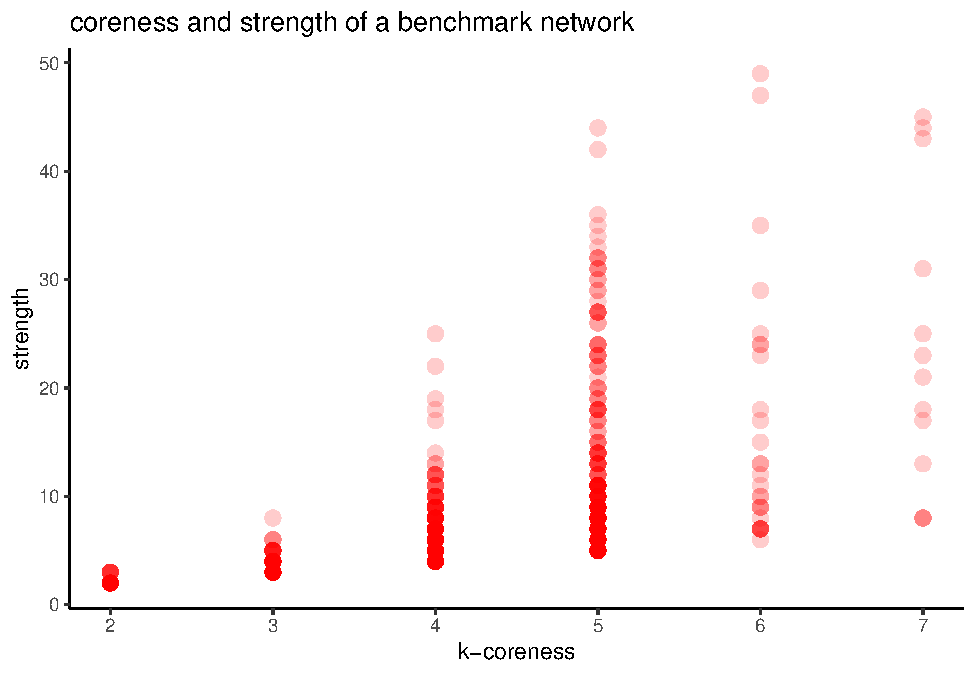
\includegraphics{com_det_algorithms_files/figure-latex/scatter Kcore-Sterngth benchmark-1.pdf}

\begin{Shaded}
\begin{Highlighting}[]
\NormalTok{dg }\OtherTok{\textless{}{-}}  \FunctionTok{degree}\NormalTok{(g)}
\NormalTok{ncd\_data }\OtherTok{\textless{}{-}} \FunctionTok{data.frame}\NormalTok{(}\AttributeTok{d =}\NormalTok{ dg, }\AttributeTok{nc =} \FunctionTok{as.factor}\NormalTok{(}\FunctionTok{V}\NormalTok{(g)}\SpecialCharTok{$}\NormalTok{community))}
\NormalTok{ncd\_data }\SpecialCharTok{\%\textgreater{}\%} \FunctionTok{ggplot}\NormalTok{(}\FunctionTok{aes}\NormalTok{(}\AttributeTok{x =}\NormalTok{ d, }\AttributeTok{y =}\NormalTok{ nc, }\AttributeTok{color =}\NormalTok{ nc))}\SpecialCharTok{+}
  \FunctionTok{geom\_vline}\NormalTok{(}\AttributeTok{xintercept =} \FunctionTok{mean}\NormalTok{(dg),  }\AttributeTok{color =} \StringTok{\textquotesingle{}black\textquotesingle{}}\NormalTok{, }\AttributeTok{linewidth =} \DecValTok{1}\NormalTok{, }\AttributeTok{alpha =} \DecValTok{1}\NormalTok{)}\SpecialCharTok{+}
  \FunctionTok{geom\_point}\NormalTok{( }\AttributeTok{size =} \DecValTok{3}\NormalTok{, }\AttributeTok{alpha =}\NormalTok{ .}\DecValTok{2}\NormalTok{)}\SpecialCharTok{+}
  \FunctionTok{labs}\NormalTok{(}\AttributeTok{title =} \StringTok{"built{-}in communities"}\NormalTok{, }\AttributeTok{x =} \StringTok{"degree"}\NormalTok{, }\AttributeTok{y =} \StringTok{"community ID"}\NormalTok{) }\SpecialCharTok{+}     \FunctionTok{theme\_classic}\NormalTok{() }
\end{Highlighting}
\end{Shaded}

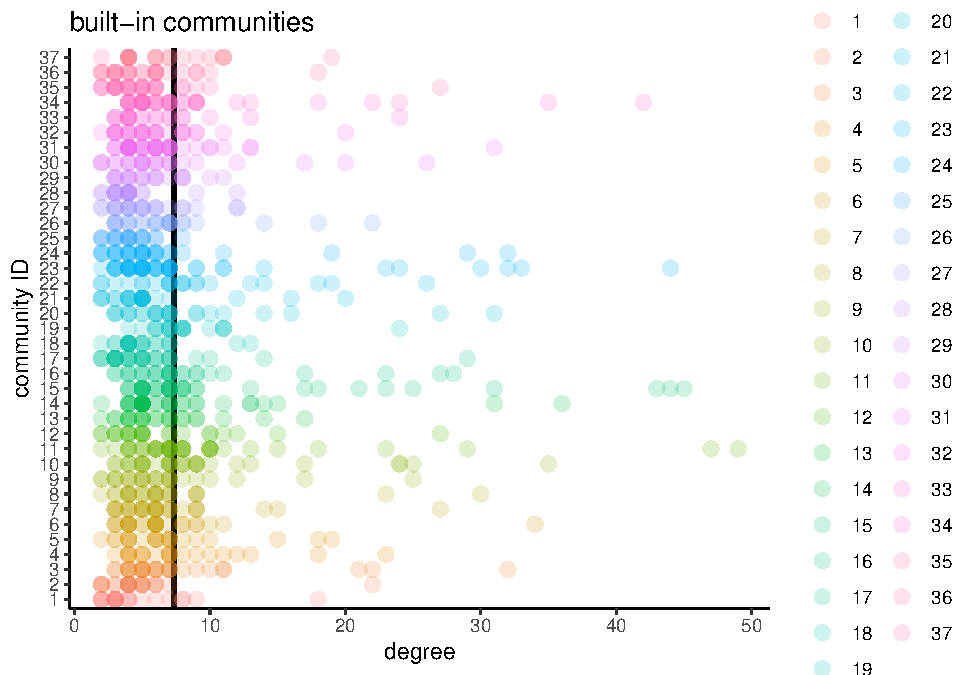
\includegraphics{com_det_algorithms_files/figure-latex/scatter nc degree-1.pdf}

The family of benchmark networks can be characterized by the modularity
of its built-in communities.

\begin{Shaded}
\begin{Highlighting}[]
\NormalTok{mod\_benchmarks }\OtherTok{\textless{}{-}} \FunctionTok{data.frame}\NormalTok{(}\AttributeTok{method =} \FunctionTok{character}\NormalTok{(), }\AttributeTok{mu =} \FunctionTok{numeric}\NormalTok{(), }\AttributeTok{modularity =} \FunctionTok{numeric}\NormalTok{())}
\NormalTok{method }\OtherTok{\textless{}{-}} \StringTok{"built{-}in"}
\ControlFlowTok{for}\NormalTok{ (mu }\ControlFlowTok{in} \FunctionTok{seq}\NormalTok{(}\DecValTok{10}\NormalTok{, }\DecValTok{70}\NormalTok{, }\DecValTok{5}\NormalTok{)) \{}
\NormalTok{    g }\OtherTok{\textless{}{-}} \FunctionTok{load\_benchmark\_network}\NormalTok{(}\AttributeTok{mui =}\NormalTok{ mu, }\AttributeTok{path =}\NormalTok{ path)}
\NormalTok{    mod }\OtherTok{\textless{}{-}} \FunctionTok{modularity}\NormalTok{(g, }\FunctionTok{make\_clusters}\NormalTok{(g,}\FunctionTok{V}\NormalTok{(g)}\SpecialCharTok{$}\NormalTok{community}\SpecialCharTok{+}\DecValTok{1}\NormalTok{ )}\SpecialCharTok{$}\NormalTok{membership )}
\NormalTok{    mod\_benchmarks }\OtherTok{\textless{}{-}} \FunctionTok{rbind}\NormalTok{(mod\_benchmarks, }\FunctionTok{data.frame}\NormalTok{(method,mu, mod))}
\NormalTok{\}}
\NormalTok{mod\_benchmarks }\SpecialCharTok{\%\textgreater{}\%} 
  \FunctionTok{ggplot}\NormalTok{(}\FunctionTok{aes}\NormalTok{(}\AttributeTok{x =}\NormalTok{ mu, }\AttributeTok{y =}\NormalTok{ mod)) }\SpecialCharTok{+}
  \FunctionTok{geom\_line}\NormalTok{(}\AttributeTok{linewidth =} \DecValTok{2}\NormalTok{, }\AttributeTok{color =} \StringTok{\textquotesingle{}gray\textquotesingle{}}\NormalTok{)}\SpecialCharTok{+}
  \FunctionTok{geom\_point}\NormalTok{()}\SpecialCharTok{+}
  \FunctionTok{ylim}\NormalTok{(}\DecValTok{0}\NormalTok{,}\DecValTok{1}\NormalTok{) }\SpecialCharTok{+} \FunctionTok{theme\_classic}\NormalTok{()}
\end{Highlighting}
\end{Shaded}

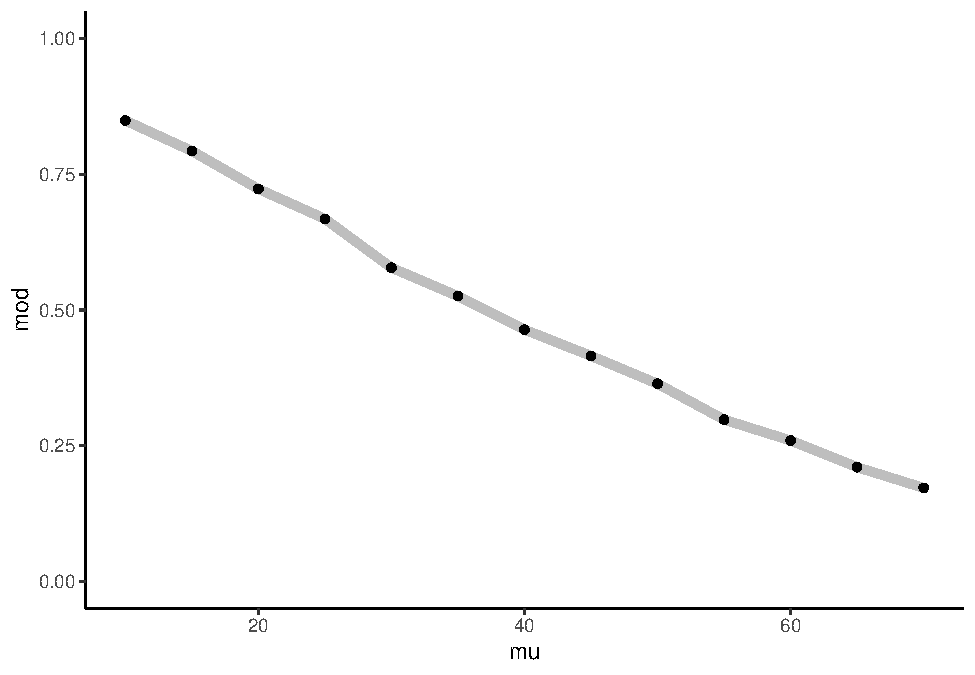
\includegraphics{com_det_algorithms_files/figure-latex/unnamed-chunk-2-1.pdf}

Methods based on modulartiy maximization are less effective with high
values of \mu.

\newpage

\hypertarget{indicators}{%
\subsection{2.2 indicators}\label{indicators}}

Modularity \(Q\) and Max(Q)that is a proxy of network fuzzyness

NMI NC number of communities NMI can be useful to measure the agreement
of two independent label assignments on the same dataset when the real
ground truth is not known.

\newpage

\hypertarget{community-definitions-and-community-detection-methods}{%
\section{3- community definitions and community detection
methods}\label{community-definitions-and-community-detection-methods}}

The definition of `community' in network analysis depends on the context
and the researcher's goals. for example:

\begin{enumerate}
\def\labelenumi{\arabic{enumi}.}
\item
  a community is a group of nodes that are more densely connected to
  each other than to the rest of the network.
\item
  a community is group of nodes that share certain characteristics, such
  as having similar properties
\item
  a community is a group of nodes that are more likely to interact with
  each other than with other nodes in the network.
\end{enumerate}

In this paper we will focus only on the first definition, and we will
test several metohds that are consisten with that definition. Namely

\begin{itemize}
\item
  FG Fast Greedy
\item
  IM infomap
\item
  LP Label Propagation
\item
  ML Multilevel (aka Louvain)
\item
  WT walktrap
\end{itemize}

\begin{Shaded}
\begin{Highlighting}[]
\NormalTok{find\_communities }\OtherTok{\textless{}{-}} \ControlFlowTok{function}\NormalTok{(g, method, }\AttributeTok{verbose =} \ConstantTok{FALSE}\NormalTok{) \{}
    \ControlFlowTok{if}\NormalTok{ (method }\SpecialCharTok{==} \StringTok{"LV"}\NormalTok{)\{}
\NormalTok{        comms }\OtherTok{\textless{}{-}} \FunctionTok{cluster\_louvain}\NormalTok{(g, }\AttributeTok{resolution =} \FloatTok{1.0}\NormalTok{)}
\NormalTok{    \} }\ControlFlowTok{else} \ControlFlowTok{if}\NormalTok{ (method }\SpecialCharTok{==} \StringTok{"FG"}\NormalTok{)\{}
\NormalTok{        comms }\OtherTok{\textless{}{-}} \FunctionTok{fastgreedy.community}\NormalTok{(g)}
\NormalTok{    \} }\ControlFlowTok{else} \ControlFlowTok{if}\NormalTok{ (method }\SpecialCharTok{==} \StringTok{"IM"}\NormalTok{)\{}
\NormalTok{        comms }\OtherTok{\textless{}{-}} \FunctionTok{infomap.community}\NormalTok{(g)}
\NormalTok{    \} }\ControlFlowTok{else} \ControlFlowTok{if}\NormalTok{ (method }\SpecialCharTok{==} \StringTok{"LP"}\NormalTok{)\{}
\NormalTok{        comms }\OtherTok{\textless{}{-}} \FunctionTok{label.propagation.community}\NormalTok{(g)}
\NormalTok{    \} }\ControlFlowTok{else} \ControlFlowTok{if}\NormalTok{ (method }\SpecialCharTok{==} \StringTok{"ML"}\NormalTok{)\{}
\NormalTok{        comms }\OtherTok{\textless{}{-}} \FunctionTok{multilevel.community}\NormalTok{(g)}
\NormalTok{    \} }\ControlFlowTok{else} \ControlFlowTok{if}\NormalTok{ (method }\SpecialCharTok{==} \StringTok{"WT"}\NormalTok{)\{}
\NormalTok{        comms }\OtherTok{\textless{}{-}} \FunctionTok{walktrap.community}\NormalTok{(g)}
\NormalTok{    \} }\ControlFlowTok{else}\NormalTok{ \{}
        \FunctionTok{print}\NormalTok{(}\StringTok{"No valid method"}\NormalTok{)}
\NormalTok{        stop}
\NormalTok{    \}}
\NormalTok{    comms}\SpecialCharTok{$}\NormalTok{algorithm }\OtherTok{=}\NormalTok{ method}
    \ControlFlowTok{if}\NormalTok{ (verbose }\SpecialCharTok{==} \ConstantTok{TRUE}\NormalTok{) \{}\FunctionTok{print}\NormalTok{(}\FunctionTok{paste}\NormalTok{(}\StringTok{"Community detection with "}\NormalTok{, method, }\StringTok{"completed."}\NormalTok{))\}}
    \FunctionTok{return}\NormalTok{(comms)}
\NormalTok{\}}
\end{Highlighting}
\end{Shaded}

Each method will be explored separately, in a single trial on a LFR
benchmark network, highlighting the main results with the followin
gfunction

\begin{Shaded}
\begin{Highlighting}[]
\NormalTok{analyse\_communities }\OtherTok{\textless{}{-}} \ControlFlowTok{function}\NormalTok{(communities, mui, }\AttributeTok{verbose =} \ConstantTok{FALSE}\NormalTok{)\{}
\NormalTok{    method }\OtherTok{\textless{}{-}}\NormalTok{ communities}\SpecialCharTok{$}\NormalTok{algorithm}
\NormalTok{    c\_membership }\OtherTok{\textless{}{-}}\NormalTok{ communities}\SpecialCharTok{$}\NormalTok{membership}
\NormalTok{    mod }\OtherTok{\textless{}{-}} \FunctionTok{round}\NormalTok{(}\FunctionTok{modularity}\NormalTok{ (g,  c\_membership}\SpecialCharTok{+}\DecValTok{1}\NormalTok{), }\AttributeTok{digits =} \DecValTok{4}\NormalTok{)}
    \CommentTok{\# need to use c\_membership + 1 to handle community label 0}
\NormalTok{    nc }\OtherTok{\textless{}{-}} \FunctionTok{length}\NormalTok{(}\FunctionTok{table}\NormalTok{(c\_membership))}
    \CommentTok{\# NMI against "Built In Communities"}
\NormalTok{    nmi }\OtherTok{=} \FunctionTok{round}\NormalTok{(aricode}\SpecialCharTok{::}\FunctionTok{NMI}\NormalTok{( }\FunctionTok{as.factor}\NormalTok{(}\FunctionTok{V}\NormalTok{(g)}\SpecialCharTok{$}\NormalTok{community),}\FunctionTok{as.factor}\NormalTok{(c\_membership)), }\DecValTok{3}\NormalTok{)}
    \ControlFlowTok{if}\NormalTok{(verbose }\SpecialCharTok{==} \ConstantTok{TRUE}\NormalTok{)\{}
        \FunctionTok{print}\NormalTok{(}\FunctionTok{paste}\NormalTok{(}\StringTok{"Communities found: "}\NormalTok{,nc))}
        \FunctionTok{print}\NormalTok{(}\FunctionTok{paste}\NormalTok{(}\StringTok{"Modularity: "}\NormalTok{, mod))}
        \FunctionTok{print}\NormalTok{(}\FunctionTok{paste}\NormalTok{(}\StringTok{"Normalized Mutual Information between C.D. method and built{-}in communities:"}\NormalTok{, nmi))}
\NormalTok{    \} }
    \FunctionTok{return}\NormalTok{(}\FunctionTok{data.frame}\NormalTok{(mui, method , mod, nc, nmi))}
\NormalTok{\}}
\end{Highlighting}
\end{Shaded}

all trials use the same network

\begin{Shaded}
\begin{Highlighting}[]
\NormalTok{mui }\OtherTok{=} \DecValTok{30}
\NormalTok{g }\OtherTok{\textless{}{-}} \FunctionTok{load\_benchmark\_network}\NormalTok{(}\AttributeTok{mui =}\NormalTok{ mui, }\AttributeTok{path =}\NormalTok{ path, }\AttributeTok{verbose =} \ConstantTok{TRUE}\NormalTok{)}
\end{Highlighting}
\end{Shaded}

\begin{verbatim}
## [1] "Loaded benchmark network ./LFR_graphs/LFR/LFR_benchmark_30.gml"
## [1] "Giant component size : 1000"
## [1] "Built-in communities:  37"
## [1] "Modularity of built-in communities:  0.5778"
\end{verbatim}

\newpage

\hypertarget{method-fg-fast-greedy}{%
\subsection{3.1 Method FG Fast Greedy}\label{method-fg-fast-greedy}}

This algorithm was proposed by Clauset et al.12. It is a greedy
community analysis algorithm that optimises the modularity score. This
method starts with a totally non-clustered initial assignment, where
each node forms a singleton community, and then computes the expected
improvement of modularity for each pair of communities, chooses a
community pair that gives the maximum improvement of modularity and
merges them into a new community. The above procedure is repeated until
no community pairs merge leads to an increase in modularity. For sparse,
hierarchical, networks the algorithm runs in \(O\)(N log2(N)).

\begin{Shaded}
\begin{Highlighting}[]
\NormalTok{g }\OtherTok{\textless{}{-}} \FunctionTok{load\_benchmark\_network}\NormalTok{(}\AttributeTok{mui =}\NormalTok{ mui, }\AttributeTok{path =}\NormalTok{ path)}
\NormalTok{tmp\_comms }\OtherTok{\textless{}{-}} \FunctionTok{find\_communities}\NormalTok{(g, }\AttributeTok{method =} \StringTok{"FG"}\NormalTok{, }\AttributeTok{verbose =} \ConstantTok{FALSE}\NormalTok{)}
\NormalTok{results }\OtherTok{\textless{}{-}} \FunctionTok{analyse\_communities}\NormalTok{(tmp\_comms, mui, }\AttributeTok{verbose =} \ConstantTok{TRUE}\NormalTok{)}
\end{Highlighting}
\end{Shaded}

\begin{verbatim}
## [1] "Communities found:  13"
## [1] "Modularity:  0.5539"
## [1] "Normalized Mutual Information between C.D. method and built-in communities: 0.489"
\end{verbatim}

\hypertarget{method-im-infomap}{%
\subsection{3.2 Method IM infomap}\label{method-im-infomap}}

This algorithm was proposed by Rosvall et al.35,36. It figures out
communities by employing random walks to analyse the information flow
through a network17. This algorithm starts with encoding the network
into modules in a way that maximises the amount of information about the
original network. Then it sends the signal to a decoder through a
channel with limited capacity. The decoder tries to decode the message
and to construct a set of possible candidates for the original graph.
The smaller the number of candidates, the more information about the
original network has been transferred. This algorithm runs in \(O\)(E).

\begin{Shaded}
\begin{Highlighting}[]
\NormalTok{tmp\_comms }\OtherTok{\textless{}{-}} \FunctionTok{find\_communities}\NormalTok{(g, }\AttributeTok{method =} \StringTok{"IM"}\NormalTok{, }\AttributeTok{verbose =} \ConstantTok{FALSE}\NormalTok{)}
\NormalTok{results }\OtherTok{\textless{}{-}} \FunctionTok{analyse\_communities}\NormalTok{(tmp\_comms, mui, }\AttributeTok{verbose =} \ConstantTok{TRUE}\NormalTok{)}
\end{Highlighting}
\end{Shaded}

\begin{verbatim}
## [1] "Communities found:  59"
## [1] "Modularity:  0.5856"
## [1] "Normalized Mutual Information between C.D. method and built-in communities: 0.845"
\end{verbatim}

\hypertarget{method-lp-label-propagation}{%
\subsection{3.3 method LP Label
Propagation}\label{method-lp-label-propagation}}

This algorithm was introduced by Raghavan et al.38. It assumes that each
node in the network is assigned to the same community as the majority of
its neighbours. This algorithm starts with initialising a distinct label
(community) for each node in the network. Then, the nodes in the network
are listed in a random sequential order. Afterwards, through the
sequence, each node takes the label of the majority of its neighbours.
The above step will stop once each node has the same label as the
majority of its neighbours. The computational complexity of label
propagation algorithm is \(O\)(E).

\begin{Shaded}
\begin{Highlighting}[]
\NormalTok{g }\OtherTok{\textless{}{-}} \FunctionTok{load\_benchmark\_network}\NormalTok{(}\AttributeTok{mui =}\NormalTok{ mui, }\AttributeTok{path =}\NormalTok{ path)}
\NormalTok{tmp\_comms }\OtherTok{\textless{}{-}} \FunctionTok{find\_communities}\NormalTok{(g, }\AttributeTok{method =} \StringTok{"IM"}\NormalTok{, }\AttributeTok{verbose =} \ConstantTok{FALSE}\NormalTok{)}
\NormalTok{results }\OtherTok{\textless{}{-}} \FunctionTok{analyse\_communities}\NormalTok{(tmp\_comms, mui, }\AttributeTok{verbose =} \ConstantTok{TRUE}\NormalTok{)}
\end{Highlighting}
\end{Shaded}

\begin{verbatim}
## [1] "Communities found:  56"
## [1] "Modularity:  0.5853"
## [1] "Normalized Mutual Information between C.D. method and built-in communities: 0.841"
\end{verbatim}

\hypertarget{method-ml-multilevel-louvain}{%
\subsection{3.4 method ML Multilevel
(Louvain)}\label{method-ml-multilevel-louvain}}

This algorithm was introduced by Blondel et al.. It is a different
greedy approach for optimising the modularity with respect to the
Fastgreedy method. This method first assigns a different community to
each node of the network, then a node is moved to the community of one
of its neighbours with which it achieves the highest positive
contribution to modularity. The above step is repeated for all nodes
until no further improvement can be achieved. Then each community is
considered as a single node on its own and the second step is repeated
until there is only a single node left or when the modularity can't be
increased in a single step. The computational complexity of the
Multilevel algorithm is \(O\)(N log N). Blondel, V. D., Guillaume,
J.-L., Lambiotte, R. \& Lefebvre, E. Fast unfolding of communities in
large networks. Journal of Statistical Mechanics: Theory and Experiment
2008, P10008 (2008).

\begin{Shaded}
\begin{Highlighting}[]
\NormalTok{g }\OtherTok{\textless{}{-}} \FunctionTok{load\_benchmark\_network}\NormalTok{(}\AttributeTok{mui =}\NormalTok{ mui, }\AttributeTok{path =}\NormalTok{ path)}
\NormalTok{tmp\_comms }\OtherTok{\textless{}{-}} \FunctionTok{find\_communities}\NormalTok{(g, }\AttributeTok{method =} \StringTok{"ML"}\NormalTok{, }\AttributeTok{verbose =} \ConstantTok{FALSE}\NormalTok{)}
\NormalTok{results }\OtherTok{\textless{}{-}} \FunctionTok{analyse\_communities}\NormalTok{(tmp\_comms, mui, }\AttributeTok{verbose =} \ConstantTok{TRUE}\NormalTok{)}
\end{Highlighting}
\end{Shaded}

\begin{verbatim}
## [1] "Communities found:  22"
## [1] "Modularity:  0.5901"
## [1] "Normalized Mutual Information between C.D. method and built-in communities: 0.697"
\end{verbatim}

\hypertarget{method-wt-walktrap}{%
\subsection{3.5 method WT walktrap}\label{method-wt-walktrap}}

This algorithm was proposed by Pon \& Latapy. It is a hierarchical
clustering algorithm. The basic idea of this method is that short
distance random walks tend to stay in the same community. Starting from
a totally non-clustered partition, the distances between all adjacent
nodes are computed. Then, two adjacent communities are chosen, they are
merged into a new one and the distances between communities are updated.
This step is repeated (N-1) times, thus the computational complexity of
this algorithm is \(O\)(E N2). For sparse networks the computational
complexity is \(O\)(N2 log(N)

\begin{Shaded}
\begin{Highlighting}[]
\NormalTok{g }\OtherTok{\textless{}{-}} \FunctionTok{load\_benchmark\_network}\NormalTok{(}\AttributeTok{mui =}\NormalTok{ mui, }\AttributeTok{path =}\NormalTok{ path)}
\NormalTok{tmp\_comms }\OtherTok{\textless{}{-}} \FunctionTok{find\_communities}\NormalTok{(g, }\AttributeTok{method =} \StringTok{"WT"}\NormalTok{, }\AttributeTok{verbose =} \ConstantTok{FALSE}\NormalTok{)}
\NormalTok{results }\OtherTok{\textless{}{-}} \FunctionTok{analyse\_communities}\NormalTok{(tmp\_comms, mui, }\AttributeTok{verbose =} \ConstantTok{TRUE}\NormalTok{)}
\end{Highlighting}
\end{Shaded}

\begin{verbatim}
## [1] "Communities found:  46"
## [1] "Modularity:  0.5689"
## [1] "Normalized Mutual Information between C.D. method and built-in communities: 0.761"
\end{verbatim}

\newpage

\hypertarget{performance-of-6-cd-methods-on-lfr-benchmark-networks-repeated-trials}{%
\section{4- performance of 6 CD methods on LFR benchmark networks
(repeated
trials)}\label{performance-of-6-cd-methods-on-lfr-benchmark-networks-repeated-trials}}

Exploring the variations of results: we generate 200 trials for a range
of MU and save results in a csv file.

\begin{Shaded}
\begin{Highlighting}[]
\NormalTok{summary\_results}\OtherTok{\textless{}{-}} \FunctionTok{read\_csv}\NormalTok{(}\StringTok{\textquotesingle{}n\_trials\_summary\_results.csv\textquotesingle{}}\NormalTok{)  }
\NormalTok{membership\_matrix }\OtherTok{\textless{}{-}} \FunctionTok{as.matrix}\NormalTok{(}\FunctionTok{read\_csv}\NormalTok{(}\StringTok{\textquotesingle{}n\_trials\_membership.csv\textquotesingle{}}\NormalTok{))}
\end{Highlighting}
\end{Shaded}

\hypertarget{performance-of-different-methods-over-repeated-trials-modularity}{%
\subsection{4.1 performance of different methods over repeated trials:
modularity}\label{performance-of-different-methods-over-repeated-trials-modularity}}

\begin{Shaded}
\begin{Highlighting}[]
\NormalTok{mod\_to\_plot }\SpecialCharTok{\%\textgreater{}\%}
  \FunctionTok{ggplot}\NormalTok{(}\FunctionTok{aes}\NormalTok{(}\AttributeTok{x =}\NormalTok{ mu, }\AttributeTok{y =}\NormalTok{ mod)) }\SpecialCharTok{+}
  \FunctionTok{geom\_rect}\NormalTok{( }\FunctionTok{aes}\NormalTok{(}\ConstantTok{NULL}\NormalTok{, }\ConstantTok{NULL}\NormalTok{, }\AttributeTok{xmin =} \DecValTok{10}\NormalTok{ , }\AttributeTok{xmax =} \DecValTok{35}\NormalTok{, }\AttributeTok{ymin =} \DecValTok{0}\NormalTok{, }\AttributeTok{ymax =} \DecValTok{1}\NormalTok{ ), }\AttributeTok{fill =} \StringTok{"green"}\NormalTok{, }\AttributeTok{alpha =} \FloatTok{0.005}\NormalTok{)}\SpecialCharTok{+}
  \FunctionTok{geom\_rect}\NormalTok{( }\FunctionTok{aes}\NormalTok{(}\ConstantTok{NULL}\NormalTok{, }\ConstantTok{NULL}\NormalTok{, }\AttributeTok{xmin =} \DecValTok{35}\NormalTok{, }\AttributeTok{xmax =} \DecValTok{50}\NormalTok{, }\AttributeTok{ymin =} \DecValTok{0}\NormalTok{, }\AttributeTok{ymax =} \DecValTok{1}\NormalTok{ ), }\AttributeTok{fill =} \StringTok{"lightblue"}\NormalTok{, }\AttributeTok{alpha =} \FloatTok{0.01}\NormalTok{)}\SpecialCharTok{+}
  \FunctionTok{geom\_rect}\NormalTok{( }\FunctionTok{aes}\NormalTok{(}\ConstantTok{NULL}\NormalTok{, }\ConstantTok{NULL}\NormalTok{, }\AttributeTok{xmin =} \DecValTok{50}\NormalTok{, }\AttributeTok{xmax =} \DecValTok{70}\NormalTok{, }\AttributeTok{ymin =} \DecValTok{0}\NormalTok{, }\AttributeTok{ymax =} \DecValTok{1}\NormalTok{ ), }\AttributeTok{fill =} \StringTok{"yellow"}\NormalTok{, }\AttributeTok{alpha =} \FloatTok{0.005}\NormalTok{)}\SpecialCharTok{+}
  \FunctionTok{geom\_line}\NormalTok{(}\AttributeTok{data =} \FunctionTok{subset}\NormalTok{(mod\_to\_plot, method }\SpecialCharTok{!=} \StringTok{\textquotesingle{}built{-}in\textquotesingle{}}\NormalTok{), }\FunctionTok{aes}\NormalTok{(}\AttributeTok{color =}\NormalTok{ method)) }\SpecialCharTok{+}
  \FunctionTok{geom\_line}\NormalTok{(}\AttributeTok{data =} \FunctionTok{subset}\NormalTok{(mod\_to\_plot, method }\SpecialCharTok{==} \StringTok{\textquotesingle{}built{-}in\textquotesingle{}}\NormalTok{), }\AttributeTok{size =} \DecValTok{2}\NormalTok{, }\AttributeTok{color =} \StringTok{\textquotesingle{}gray\textquotesingle{}}\NormalTok{) }\SpecialCharTok{+}
  \FunctionTok{geom\_point}\NormalTok{(}\AttributeTok{data =} \FunctionTok{subset}\NormalTok{(mod\_to\_plot, method }\SpecialCharTok{!=} \StringTok{\textquotesingle{}built{-}in\textquotesingle{}}\NormalTok{), }\FunctionTok{aes}\NormalTok{(}\AttributeTok{color =}\NormalTok{ method)) }\SpecialCharTok{+}
  \FunctionTok{geom\_point}\NormalTok{(}\AttributeTok{data =} \FunctionTok{subset}\NormalTok{(mod\_to\_plot, method }\SpecialCharTok{==} \StringTok{\textquotesingle{}built{-}in\textquotesingle{}}\NormalTok{), }\AttributeTok{size =} \DecValTok{1}\NormalTok{, }\AttributeTok{color =} \StringTok{\textquotesingle{}black\textquotesingle{}}\NormalTok{) }\SpecialCharTok{+}
  
     \FunctionTok{geom\_hline}\NormalTok{(}\AttributeTok{yintercept =} \FloatTok{0.5}\NormalTok{)}\SpecialCharTok{+}
    \FunctionTok{labs}\NormalTok{(}\AttributeTok{title =} \StringTok{"performance of different methods (modularity)"}\NormalTok{, }\AttributeTok{y =} \StringTok{"modularity"}\NormalTok{, }\AttributeTok{x =} \StringTok{"mu"}\NormalTok{) }\SpecialCharTok{+}
    \FunctionTok{theme\_light}\NormalTok{()   }
\end{Highlighting}
\end{Shaded}

\begin{verbatim}
## Warning: Using `size` aesthetic for lines was deprecated in ggplot2 3.4.0.
## i Please use `linewidth` instead.
\end{verbatim}

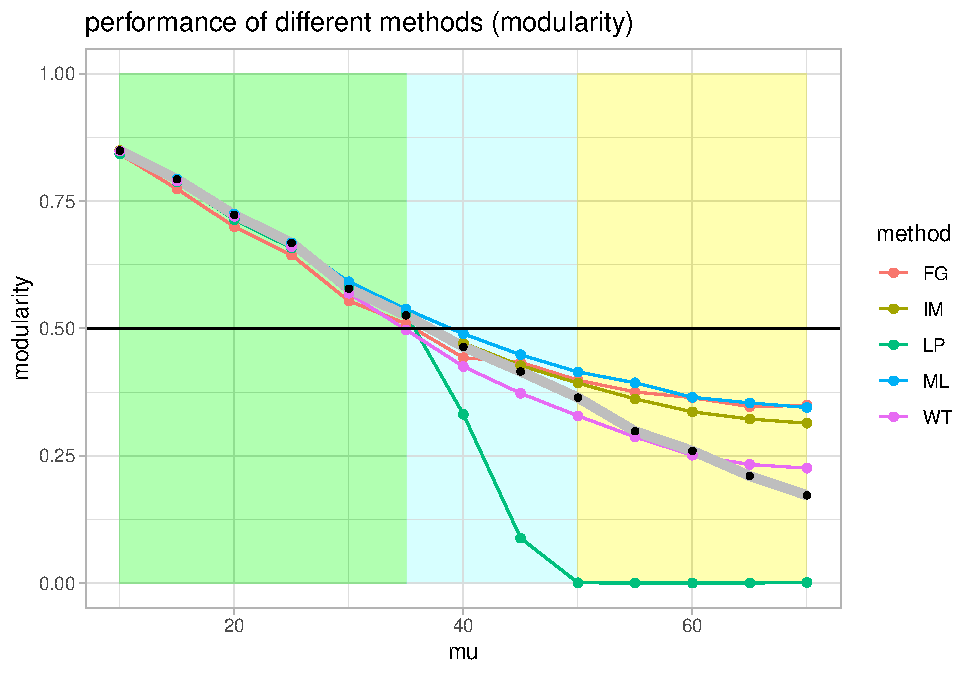
\includegraphics{com_det_algorithms_files/figure-latex/unnamed-chunk-10-1.pdf}

Note that when modularity \textless{} 0.5, the definition of community
is not consistent. WHen LP returns modularity \textgreater{} 0.5 it is
very accurate. returns modularity \textless{} 0.5, the algorithm fails.
This is a very relevant insight try modularity / modularityBI

\begin{Shaded}
\begin{Highlighting}[]
\NormalTok{mod\_to\_plot }\SpecialCharTok{\%\textgreater{}\%} \FunctionTok{filter}\NormalTok{(method }\SpecialCharTok{!=} \StringTok{\textquotesingle{}built{-}in\textquotesingle{}}\NormalTok{) }\SpecialCharTok{\%\textgreater{}\%}
  \FunctionTok{ggplot}\NormalTok{(}\FunctionTok{aes}\NormalTok{(}\AttributeTok{x =}\NormalTok{ mu, }\AttributeTok{y =}\NormalTok{ nm)) }\SpecialCharTok{+}
  \FunctionTok{geom\_rect}\NormalTok{( }\FunctionTok{aes}\NormalTok{(}\ConstantTok{NULL}\NormalTok{, }\ConstantTok{NULL}\NormalTok{, }\AttributeTok{xmin =} \DecValTok{10}\NormalTok{ , }\AttributeTok{xmax =} \DecValTok{35}\NormalTok{, }\AttributeTok{ymin =} \DecValTok{0}\NormalTok{, }\AttributeTok{ymax =} \DecValTok{2}\NormalTok{ ), }\AttributeTok{fill =} \StringTok{"green"}\NormalTok{, }\AttributeTok{alpha =} \FloatTok{0.005}\NormalTok{)}\SpecialCharTok{+}
  \FunctionTok{geom\_rect}\NormalTok{( }\FunctionTok{aes}\NormalTok{(}\ConstantTok{NULL}\NormalTok{, }\ConstantTok{NULL}\NormalTok{, }\AttributeTok{xmin =} \DecValTok{35}\NormalTok{, }\AttributeTok{xmax =} \DecValTok{50}\NormalTok{, }\AttributeTok{ymin =} \DecValTok{0}\NormalTok{, }\AttributeTok{ymax =} \DecValTok{2}\NormalTok{ ), }\AttributeTok{fill =} \StringTok{"lightblue"}\NormalTok{, }\AttributeTok{alpha =} \FloatTok{0.01}\NormalTok{)}\SpecialCharTok{+}
  \FunctionTok{geom\_rect}\NormalTok{( }\FunctionTok{aes}\NormalTok{(}\ConstantTok{NULL}\NormalTok{, }\ConstantTok{NULL}\NormalTok{, }\AttributeTok{xmin =} \DecValTok{50}\NormalTok{, }\AttributeTok{xmax =} \DecValTok{70}\NormalTok{, }\AttributeTok{ymin =} \DecValTok{0}\NormalTok{, }\AttributeTok{ymax =} \DecValTok{2}\NormalTok{ ), }\AttributeTok{fill =} \StringTok{"yellow"}\NormalTok{, }\AttributeTok{alpha =} \FloatTok{0.005}\NormalTok{)}\SpecialCharTok{+}

  \FunctionTok{geom\_line}\NormalTok{( }\FunctionTok{aes}\NormalTok{(}\AttributeTok{color =}\NormalTok{ method)) }\SpecialCharTok{+}
  \FunctionTok{geom\_point}\NormalTok{( }\FunctionTok{aes}\NormalTok{(}\AttributeTok{color =}\NormalTok{ method)) }\SpecialCharTok{+} 
    \FunctionTok{labs}\NormalTok{(}\AttributeTok{title =} \StringTok{"different performance of CD methods as a function of network fuzzynes"}\NormalTok{, }\AttributeTok{y =} \StringTok{"modularity method / modularity built{-}in"}\NormalTok{, }\AttributeTok{x =} \StringTok{"mu"}\NormalTok{) }\SpecialCharTok{+}
    \FunctionTok{theme\_minimal}\NormalTok{()   }
\end{Highlighting}
\end{Shaded}

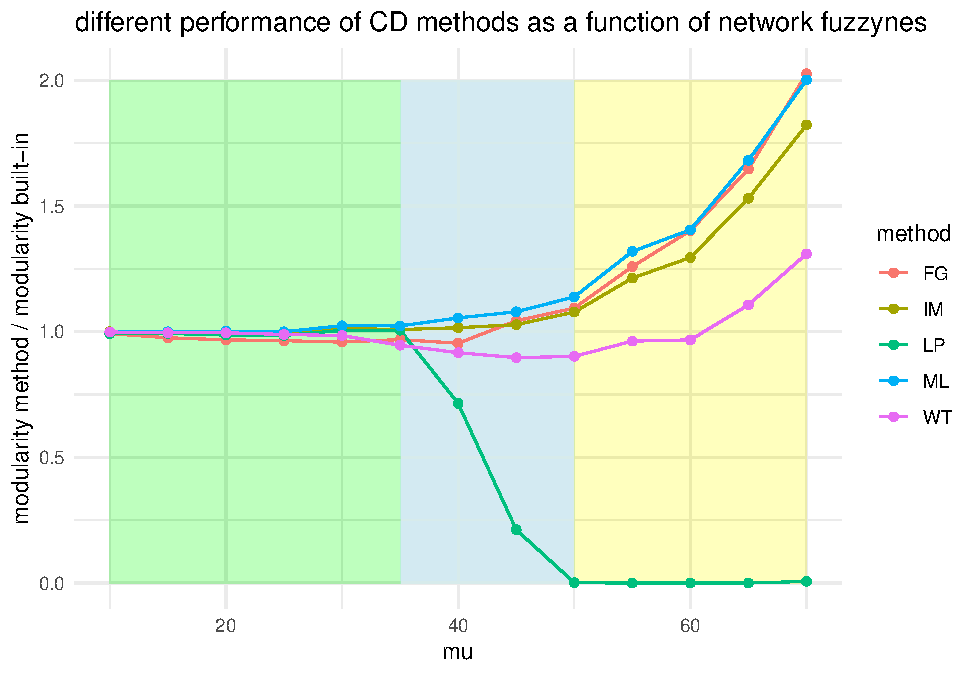
\includegraphics{com_det_algorithms_files/figure-latex/unnamed-chunk-11-1.pdf}

\hypertarget{performance-of-different-methods-over-repeated-trials-nmi}{%
\subsection{4.2 performance of different methods over repeated trials:
NMI}\label{performance-of-different-methods-over-repeated-trials-nmi}}

NMI can be calculated against the built-in communities (NMI-BI) or
against all other methods (NMI\_OM).

\begin{Shaded}
\begin{Highlighting}[]
\NormalTok{summary\_results }\SpecialCharTok{\%\textgreater{}\%} 
    \FunctionTok{filter}\NormalTok{(method }\SpecialCharTok{\%in\%} \FunctionTok{c}\NormalTok{( }\StringTok{"FG"}\NormalTok{, }\StringTok{"IM"}\NormalTok{, }\StringTok{"LP"}\NormalTok{, }\StringTok{"ML"}\NormalTok{, }\StringTok{"WT"}\NormalTok{)) }\SpecialCharTok{\%\textgreater{}\%}
  \FunctionTok{ggplot}\NormalTok{(}\FunctionTok{aes}\NormalTok{(}\AttributeTok{x =}\NormalTok{ mui, }\AttributeTok{y =}\NormalTok{ nmi)) }\SpecialCharTok{+}
    \FunctionTok{geom\_point}\NormalTok{(}\FunctionTok{aes}\NormalTok{(}\AttributeTok{color =}\NormalTok{ method)) }\SpecialCharTok{+}
    \FunctionTok{labs}\NormalTok{(}\AttributeTok{title =} \StringTok{"Performance of different methods over N trials"}\NormalTok{, }\AttributeTok{y =} \StringTok{"NMI\_BIC"}\NormalTok{, }\AttributeTok{x =} \StringTok{"mu"}\NormalTok{) }\SpecialCharTok{+}
    \FunctionTok{theme\_light}\NormalTok{()  }\SpecialCharTok{+} 
    \FunctionTok{facet\_wrap}\NormalTok{(method }\SpecialCharTok{\textasciitilde{}}\NormalTok{ .) }\CommentTok{\#,  scales = "free\_x"}
\end{Highlighting}
\end{Shaded}

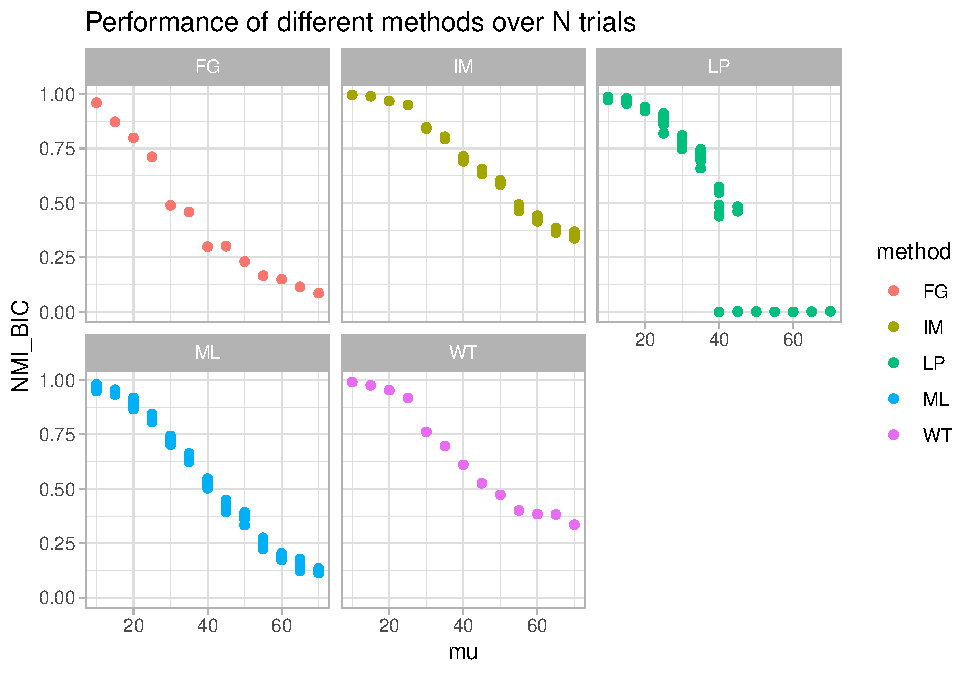
\includegraphics{com_det_algorithms_files/figure-latex/unnamed-chunk-12-1.pdf}

\begin{Shaded}
\begin{Highlighting}[]
\NormalTok{summary\_results }\SpecialCharTok{\%\textgreater{}\%} 
  \FunctionTok{filter}\NormalTok{(mui }\SpecialCharTok{\%in\%} \FunctionTok{c}\NormalTok{(}\DecValTok{40}\NormalTok{)) }\SpecialCharTok{\%\textgreater{}\%}
  \FunctionTok{filter}\NormalTok{(method }\SpecialCharTok{\%in\%} \FunctionTok{c}\NormalTok{( }\StringTok{"FG"}\NormalTok{, }\StringTok{"IM"}\NormalTok{, }\StringTok{"LP"}\NormalTok{, }\StringTok{"ML"}\NormalTok{, }\StringTok{"WT"}\NormalTok{)) }\SpecialCharTok{\%\textgreater{}\%}
    \FunctionTok{ggplot}\NormalTok{(}\FunctionTok{aes}\NormalTok{(}\AttributeTok{x =}\NormalTok{ nmi)) }\SpecialCharTok{+}
    \FunctionTok{geom\_histogram}\NormalTok{(}\AttributeTok{color =} \StringTok{"black"}\NormalTok{, }\AttributeTok{fill =} \StringTok{"red"}\NormalTok{, }\AttributeTok{bins =} \DecValTok{100}\NormalTok{) }\SpecialCharTok{+}
    \FunctionTok{labs}\NormalTok{(}\AttributeTok{title =} \StringTok{"Performance of different methods over N trials mu = 40"}\NormalTok{, }\AttributeTok{x =} \StringTok{"Normalized Mutual Information"}\NormalTok{, }\AttributeTok{y =} \StringTok{"count"}\NormalTok{) }\SpecialCharTok{+}
    \FunctionTok{geom\_vline}\NormalTok{(}\AttributeTok{xintercept =} \FloatTok{0.5}\NormalTok{, }\AttributeTok{color =} \StringTok{\textquotesingle{}red\textquotesingle{}}\NormalTok{)}\SpecialCharTok{+}
    \FunctionTok{theme\_classic}\NormalTok{() }\SpecialCharTok{+} 
    \FunctionTok{facet\_wrap}\NormalTok{(method }\SpecialCharTok{\textasciitilde{}}\NormalTok{ .)}
\end{Highlighting}
\end{Shaded}

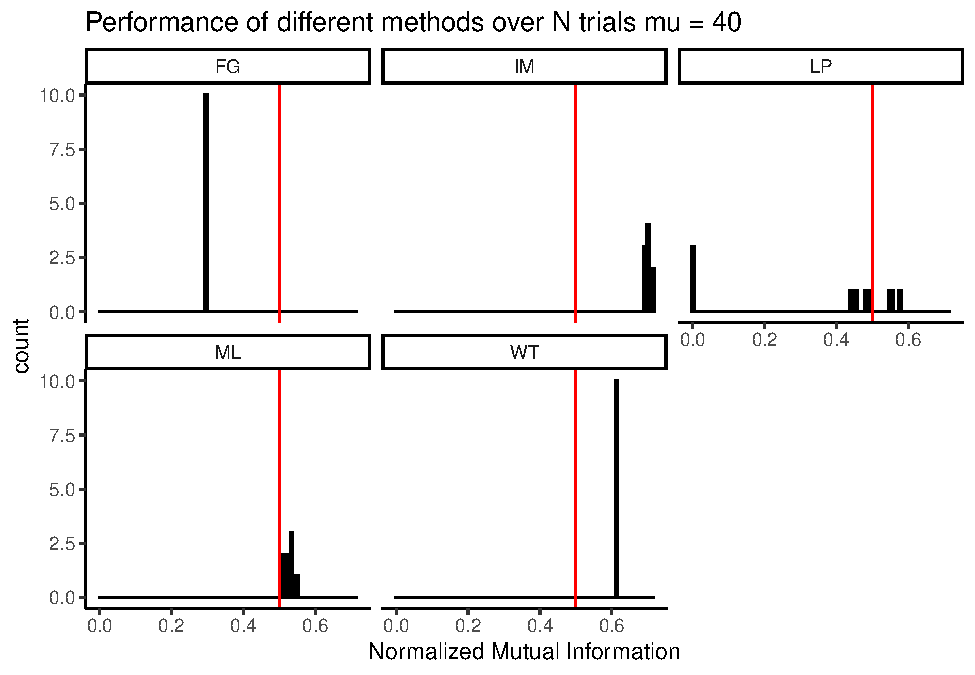
\includegraphics{com_det_algorithms_files/figure-latex/unnamed-chunk-13-1.pdf}

\newpage

The following Figure compares the results of each methods with the built
in labels, using NMI.

\begin{Shaded}
\begin{Highlighting}[]
\NormalTok{summary\_results }\SpecialCharTok{\%\textgreater{}\%} \FunctionTok{group\_by}\NormalTok{(method, mui) }\SpecialCharTok{\%\textgreater{}\%} 
    \FunctionTok{summarise}\NormalTok{(}\AttributeTok{mean\_nmi =} \FunctionTok{mean}\NormalTok{(nmi), }\AttributeTok{sd\_nmi =} \FunctionTok{sd}\NormalTok{(nmi) ) }\SpecialCharTok{\%\textgreater{}\%}
    \FunctionTok{ggplot}\NormalTok{(}\FunctionTok{aes}\NormalTok{(}\AttributeTok{x =}\NormalTok{ mui, }\AttributeTok{y =}\NormalTok{ mean\_nmi)) }\SpecialCharTok{+}
    \FunctionTok{geom\_rect}\NormalTok{( }\FunctionTok{aes}\NormalTok{(}\ConstantTok{NULL}\NormalTok{, }\ConstantTok{NULL}\NormalTok{, }\AttributeTok{xmin =} \DecValTok{10}\NormalTok{ , }\AttributeTok{xmax =} \DecValTok{35}\NormalTok{, }\AttributeTok{ymin =} \DecValTok{0}\NormalTok{, }\AttributeTok{ymax =} \DecValTok{1}\NormalTok{ ), }\AttributeTok{fill =} \StringTok{"green"}\NormalTok{, }\AttributeTok{alpha =} \FloatTok{0.005}\NormalTok{)}\SpecialCharTok{+}
    \FunctionTok{geom\_rect}\NormalTok{( }\FunctionTok{aes}\NormalTok{(}\ConstantTok{NULL}\NormalTok{, }\ConstantTok{NULL}\NormalTok{, }\AttributeTok{xmin =} \DecValTok{35}\NormalTok{, }\AttributeTok{xmax =} \DecValTok{50}\NormalTok{, }\AttributeTok{ymin =} \DecValTok{0}\NormalTok{, }\AttributeTok{ymax =} \DecValTok{1}\NormalTok{ ), }\AttributeTok{fill =} \StringTok{"lightblue"}\NormalTok{, }\AttributeTok{alpha =} \FloatTok{0.01}\NormalTok{)}\SpecialCharTok{+}
    \FunctionTok{geom\_rect}\NormalTok{( }\FunctionTok{aes}\NormalTok{(}\ConstantTok{NULL}\NormalTok{, }\ConstantTok{NULL}\NormalTok{, }\AttributeTok{xmin =} \DecValTok{50}\NormalTok{, }\AttributeTok{xmax =} \DecValTok{70}\NormalTok{, }\AttributeTok{ymin =} \DecValTok{0}\NormalTok{, }\AttributeTok{ymax =} \DecValTok{1}\NormalTok{ ), }\AttributeTok{fill =} \StringTok{"yellow"}\NormalTok{, }\AttributeTok{alpha =} \FloatTok{0.005}\NormalTok{)}\SpecialCharTok{+}
    \FunctionTok{geom\_line}\NormalTok{(}\FunctionTok{aes}\NormalTok{(}\AttributeTok{color =}\NormalTok{ method)) }\SpecialCharTok{+}
    \FunctionTok{geom\_point}\NormalTok{(}\FunctionTok{aes}\NormalTok{(}\AttributeTok{color =}\NormalTok{ method)) }\SpecialCharTok{+}
    \FunctionTok{geom\_linerange}\NormalTok{(}\FunctionTok{aes}\NormalTok{(}\AttributeTok{ymin =}\NormalTok{mean\_nmi}\SpecialCharTok{{-}}\NormalTok{sd\_nmi, }\AttributeTok{ymax =}\NormalTok{ mean\_nmi }\SpecialCharTok{+}\NormalTok{ sd\_nmi, }\AttributeTok{color =}\NormalTok{ method), }\AttributeTok{linewidth =} \DecValTok{2}\NormalTok{, }\AttributeTok{alpha =} \FloatTok{0.5}\NormalTok{)}\SpecialCharTok{+}
    \FunctionTok{geom\_hline}\NormalTok{(}\AttributeTok{yintercept =} \FloatTok{0.5}\NormalTok{)}\SpecialCharTok{+}
    \FunctionTok{labs}\NormalTok{(}\AttributeTok{title =} \StringTok{"performance of different methods "}\NormalTok{, }\AttributeTok{y =} \StringTok{"NMI\_BIC"}\NormalTok{, }\AttributeTok{x =} \StringTok{"mu"}\NormalTok{) }\SpecialCharTok{+}
    \FunctionTok{theme\_light}\NormalTok{()  }
\end{Highlighting}
\end{Shaded}

\begin{verbatim}
## `summarise()` has grouped output by 'method'. You can override using the
## `.groups` argument.
\end{verbatim}

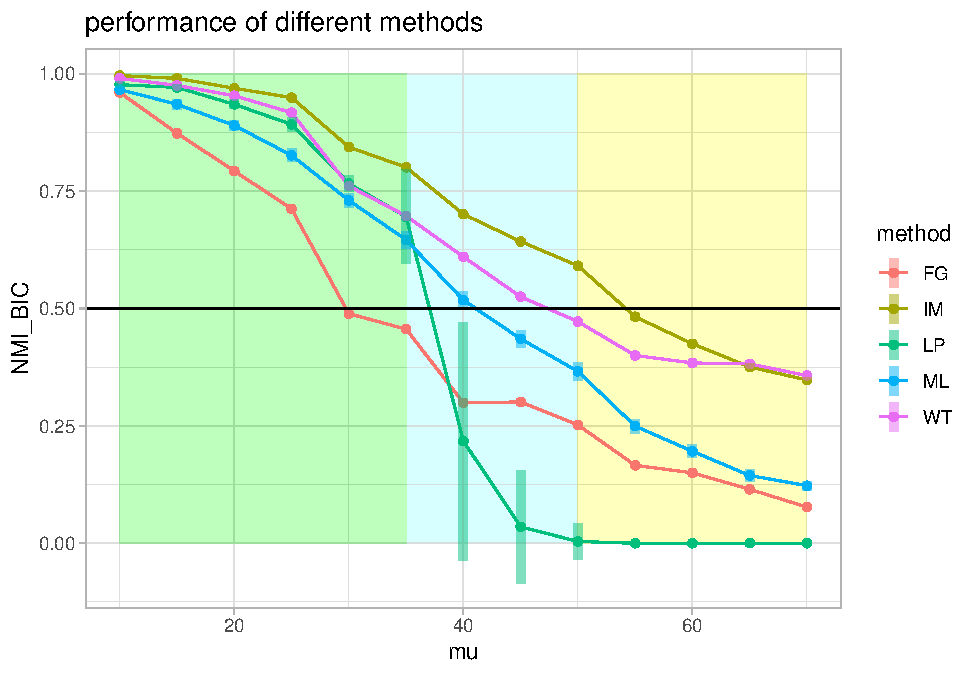
\includegraphics{com_det_algorithms_files/figure-latex/unnamed-chunk-14-1.pdf}

The following Figure compares the results of each methods with the built
in labels, using NMI.

\begin{Shaded}
\begin{Highlighting}[]
\NormalTok{summary\_results }\SpecialCharTok{\%\textgreater{}\%} \FunctionTok{group\_by}\NormalTok{(method, mui) }\SpecialCharTok{\%\textgreater{}\%} 
    \FunctionTok{summarise}\NormalTok{(}\AttributeTok{mean\_nmi =} \FunctionTok{mean}\NormalTok{(nmi), }\AttributeTok{sd\_nmi =} \FunctionTok{sd}\NormalTok{(nmi), }
              \AttributeTok{mean\_mod =} \FunctionTok{mean}\NormalTok{(mod), }\AttributeTok{sd\_mod =} \FunctionTok{sd}\NormalTok{(mod) ) }\SpecialCharTok{\%\textgreater{}\%}
    \FunctionTok{ggplot}\NormalTok{(}\FunctionTok{aes}\NormalTok{(}\AttributeTok{x =}\NormalTok{ mean\_mod, }\AttributeTok{y =}\NormalTok{ mean\_nmi)) }\SpecialCharTok{+}
    \FunctionTok{geom\_rect}\NormalTok{( }\FunctionTok{aes}\NormalTok{(}\ConstantTok{NULL}\NormalTok{, }\ConstantTok{NULL}\NormalTok{, }\AttributeTok{xmin =} \FloatTok{0.6}\NormalTok{ , }\AttributeTok{xmax =} \FloatTok{1.0}\NormalTok{, }\AttributeTok{ymin =} \DecValTok{0}\NormalTok{, }\AttributeTok{ymax =} \DecValTok{1}\NormalTok{ ), }\AttributeTok{fill =} \StringTok{"green"}\NormalTok{, }\AttributeTok{alpha =} \FloatTok{0.005}\NormalTok{)}\SpecialCharTok{+}
    \FunctionTok{geom\_rect}\NormalTok{( }\FunctionTok{aes}\NormalTok{(}\ConstantTok{NULL}\NormalTok{, }\ConstantTok{NULL}\NormalTok{, }\AttributeTok{xmin =} \FloatTok{0.35}\NormalTok{ , }\AttributeTok{xmax =} \FloatTok{0.6}\NormalTok{, }\AttributeTok{ymin =} \DecValTok{0}\NormalTok{, }\AttributeTok{ymax =} \DecValTok{1}\NormalTok{ ), }\AttributeTok{fill =} \StringTok{"lightblue"}\NormalTok{, }\AttributeTok{alpha =} \FloatTok{0.01}\NormalTok{)}\SpecialCharTok{+}
    \FunctionTok{geom\_rect}\NormalTok{( }\FunctionTok{aes}\NormalTok{(}\ConstantTok{NULL}\NormalTok{, }\ConstantTok{NULL}\NormalTok{, }\AttributeTok{xmin =} \FloatTok{0.0}\NormalTok{ , }\AttributeTok{xmax =} \FloatTok{0.35}\NormalTok{, }\AttributeTok{ymin =} \DecValTok{0}\NormalTok{, }\AttributeTok{ymax =} \DecValTok{1}\NormalTok{ ), }\AttributeTok{fill =} \StringTok{"yellow"}\NormalTok{, }\AttributeTok{alpha =} \FloatTok{0.005}\NormalTok{)}\SpecialCharTok{+}

      \FunctionTok{geom\_line}\NormalTok{(}\FunctionTok{aes}\NormalTok{(}\AttributeTok{color =}\NormalTok{ method)) }\SpecialCharTok{+}
    \FunctionTok{geom\_point}\NormalTok{(}\FunctionTok{aes}\NormalTok{(}\AttributeTok{color =}\NormalTok{ method)) }\SpecialCharTok{+}
    \CommentTok{\#geom\_linerange(aes(ymin = mean\_nmi {-} sd\_nmi, ymax = mean\_nmi + sd\_nmi, color = method), linewidth = 2, alpha = 0.5)+}
    \CommentTok{\#geom\_linerange(aes(xmin = mean\_mod {-} sd\_mod, xmax = mean\_mod + sd\_mod, color = method), linewidth = 2, alpha = 0.5)+}
      \FunctionTok{geom\_hline}\NormalTok{(}\AttributeTok{yintercept =} \FloatTok{0.5}\NormalTok{)}\SpecialCharTok{+}
    \FunctionTok{labs}\NormalTok{(}\AttributeTok{title =} \StringTok{"performance of different methods "}\NormalTok{, }\AttributeTok{y =} \StringTok{"NMI\_BIC"}\NormalTok{, }\AttributeTok{x =} \StringTok{"modularity"}\NormalTok{) }\SpecialCharTok{+}
    \FunctionTok{theme\_minimal}\NormalTok{()  }
\end{Highlighting}
\end{Shaded}

\begin{verbatim}
## `summarise()` has grouped output by 'method'. You can override using the
## `.groups` argument.
\end{verbatim}

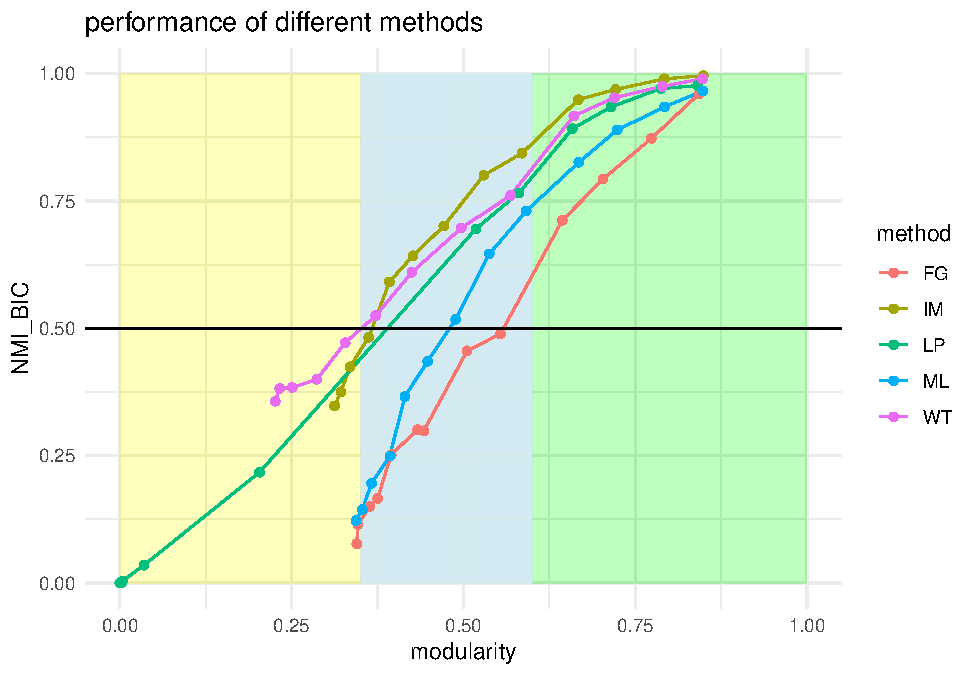
\includegraphics{com_det_algorithms_files/figure-latex/unnamed-chunk-15-1.pdf}

\begin{Shaded}
\begin{Highlighting}[]
\NormalTok{ data\_points }\OtherTok{\textless{}{-}}\NormalTok{ summary\_results}
\NormalTok{data\_lines }\OtherTok{\textless{}{-}}\NormalTok{ summary\_results }\SpecialCharTok{\%\textgreater{}\%} \FunctionTok{group\_by}\NormalTok{(method, mui) }\SpecialCharTok{\%\textgreater{}\%} 
    \FunctionTok{summarise}\NormalTok{(}\AttributeTok{mean\_nmi =} \FunctionTok{mean}\NormalTok{(nmi), }\AttributeTok{sd\_nmi =} \FunctionTok{sd}\NormalTok{(nmi), }
              \AttributeTok{mean\_mod =} \FunctionTok{mean}\NormalTok{(mod), }\AttributeTok{sd\_mod =} \FunctionTok{sd}\NormalTok{(mod) ) }
\end{Highlighting}
\end{Shaded}

\begin{verbatim}
## `summarise()` has grouped output by 'method'. You can override using the
## `.groups` argument.
\end{verbatim}

\begin{Shaded}
\begin{Highlighting}[]
\FunctionTok{ggplot}\NormalTok{() }\SpecialCharTok{+}
    \FunctionTok{geom\_line}\NormalTok{(}\AttributeTok{data =}\NormalTok{ data\_lines, }\FunctionTok{aes}\NormalTok{(}\AttributeTok{x =}\NormalTok{ mean\_mod, }\AttributeTok{y =}\NormalTok{ mean\_nmi, }\AttributeTok{color =}\NormalTok{ method)) }\SpecialCharTok{+}
    \FunctionTok{geom\_linerange}\NormalTok{(}\AttributeTok{data =}\NormalTok{ data\_lines, }\FunctionTok{aes}\NormalTok{(}\AttributeTok{x =}\NormalTok{ mean\_mod, }\AttributeTok{y =}\NormalTok{ mean\_nmi,}\AttributeTok{ymin =}\NormalTok{ mean\_nmi }\SpecialCharTok{{-}}\NormalTok{ sd\_nmi, }\AttributeTok{ymax =}\NormalTok{ mean\_nmi }\SpecialCharTok{+}\NormalTok{ sd\_nmi, }\AttributeTok{color =}\NormalTok{ method), }\AttributeTok{linewidth =} \DecValTok{2}\NormalTok{, }\AttributeTok{alpha =} \FloatTok{0.5}\NormalTok{)}\SpecialCharTok{+}
    \FunctionTok{geom\_linerange}\NormalTok{(}\AttributeTok{data =}\NormalTok{ data\_lines, }\FunctionTok{aes}\NormalTok{(}\AttributeTok{x =}\NormalTok{ mean\_mod, }\AttributeTok{y =}\NormalTok{ mean\_nmi,}\AttributeTok{xmin =}\NormalTok{ mean\_mod }\SpecialCharTok{{-}}\NormalTok{ sd\_mod, }\AttributeTok{xmax =}\NormalTok{ mean\_mod }\SpecialCharTok{+}\NormalTok{ sd\_mod, }\AttributeTok{color =}\NormalTok{ method), }\AttributeTok{linewidth =} \DecValTok{2}\NormalTok{, }\AttributeTok{alpha =} \FloatTok{0.5}\NormalTok{)}\SpecialCharTok{+}
      \FunctionTok{geom\_point}\NormalTok{(}\AttributeTok{data =}\NormalTok{ data\_points, }\FunctionTok{aes}\NormalTok{(}\AttributeTok{x =}\NormalTok{ mod, }\AttributeTok{y =}\NormalTok{ nmi, }\AttributeTok{color =}\NormalTok{ method)) }\SpecialCharTok{+}

      \FunctionTok{geom\_hline}\NormalTok{(}\AttributeTok{yintercept =} \FloatTok{0.5}\NormalTok{)}\SpecialCharTok{+}
    \FunctionTok{labs}\NormalTok{(}\AttributeTok{title =} \StringTok{"performance of different methods "}\NormalTok{, }\AttributeTok{y =} \StringTok{"NMI\_BIC"}\NormalTok{, }\AttributeTok{x =} \StringTok{"modularity"}\NormalTok{) }\SpecialCharTok{+}
    \FunctionTok{theme\_light}\NormalTok{()  }\SpecialCharTok{+} \FunctionTok{facet\_wrap}\NormalTok{(method }\SpecialCharTok{\textasciitilde{}}\NormalTok{ .)}
\end{Highlighting}
\end{Shaded}

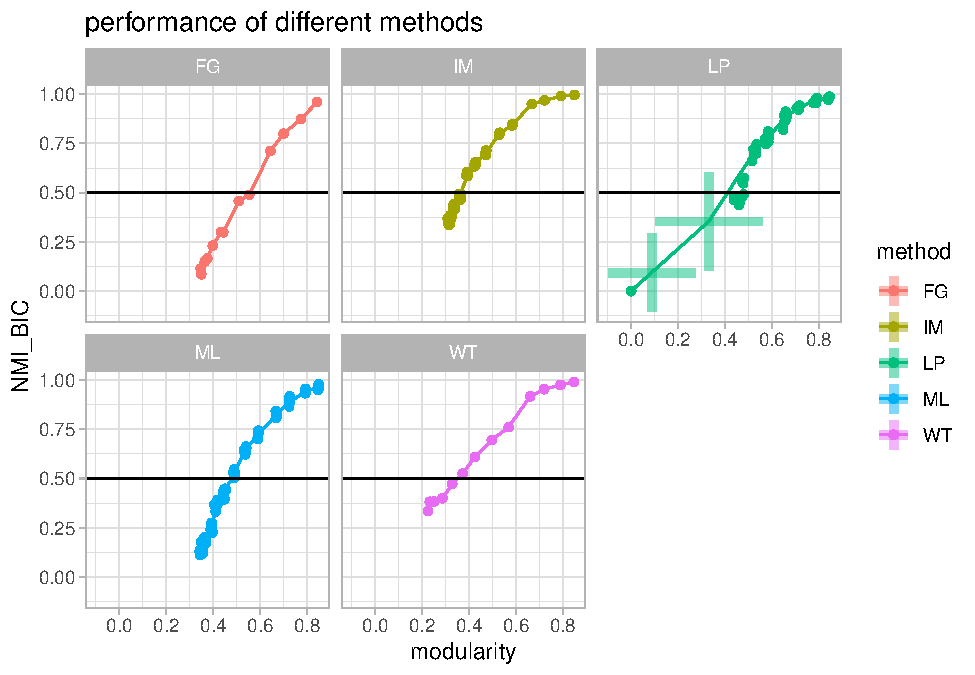
\includegraphics{com_det_algorithms_files/figure-latex/unnamed-chunk-16-1.pdf}

\newpage

\hypertarget{community-detection-to-assess-fuzzyness}{%
\subsection{community detection to assess
``fuzzyness''}\label{community-detection-to-assess-fuzzyness}}

When dealing with an unsupervised community detection task, it is
important to remember that the term ``detection'' is misleading.
Communities are not an intrinsic property of the network, but rather
arise as the result of an algorithm. The results depend on network
properties, the chosen algorithm, its parameters, and its intrinsic
stochasticity.

Additionally, networks may generate communities with different levels of
fuzziness. Low fuzziness refers to well-defined communities in which
members have strong connections with each other and weak connections to
members of other communities. High fuzziness, on the other hand, refers
to communities in which members have weaker connections with each other
and stronger connections to members of other communities. In between
these two extremes, there is a transition zone, where the strongly
fuzziness depends on the method used to measure it.

Low fuzzyness: modularity is HIGH \textgreater{} 0.5 is always high
regardless of the method. LP and FG are sensitive to fuzzyness: when
their results drop below 0.5, we are in the transition TRY NMI without
true labels

\begin{Shaded}
\begin{Highlighting}[]
\NormalTok{summary\_results }\SpecialCharTok{\%\textgreater{}\%} 
  \FunctionTok{filter}\NormalTok{(mui }\SpecialCharTok{\%in\%} \FunctionTok{c}\NormalTok{(}\DecValTok{10}\NormalTok{,}\DecValTok{20}\NormalTok{,}\DecValTok{30}\NormalTok{)) }\SpecialCharTok{\%\textgreater{}\%} 
  \FunctionTok{ggplot}\NormalTok{(}\FunctionTok{aes}\NormalTok{(}\AttributeTok{x =}\NormalTok{ mod, }\AttributeTok{y =}\NormalTok{ nmi, }\AttributeTok{color =}\NormalTok{ method)) }\SpecialCharTok{+}
  \FunctionTok{geom\_point}\NormalTok{( }\AttributeTok{size =} \DecValTok{4}\NormalTok{, }\AttributeTok{alpha =} \FloatTok{0.2}\NormalTok{) }\SpecialCharTok{+}
  \FunctionTok{geom\_vline}\NormalTok{(}\AttributeTok{xintercept =} \FloatTok{0.5}\NormalTok{, }\AttributeTok{color =} \StringTok{"red"}\NormalTok{)}\SpecialCharTok{+}
  \FunctionTok{geom\_hline}\NormalTok{(}\AttributeTok{yintercept =} \FloatTok{0.5}\NormalTok{, }\AttributeTok{color =} \StringTok{"red"}\NormalTok{)}\SpecialCharTok{+}
    \FunctionTok{labs}\NormalTok{(}\AttributeTok{title =} \StringTok{"performance of different methods LOW FUZZYNESS"}\NormalTok{, }\AttributeTok{y =} \StringTok{"NMI\_BIC"}\NormalTok{, }\AttributeTok{x =} \StringTok{"modularity"}\NormalTok{) }\SpecialCharTok{+}
  \FunctionTok{theme\_light}\NormalTok{()  }\SpecialCharTok{+} \FunctionTok{facet\_wrap}\NormalTok{(mui }\SpecialCharTok{\textasciitilde{}}\NormalTok{ .)}
\end{Highlighting}
\end{Shaded}

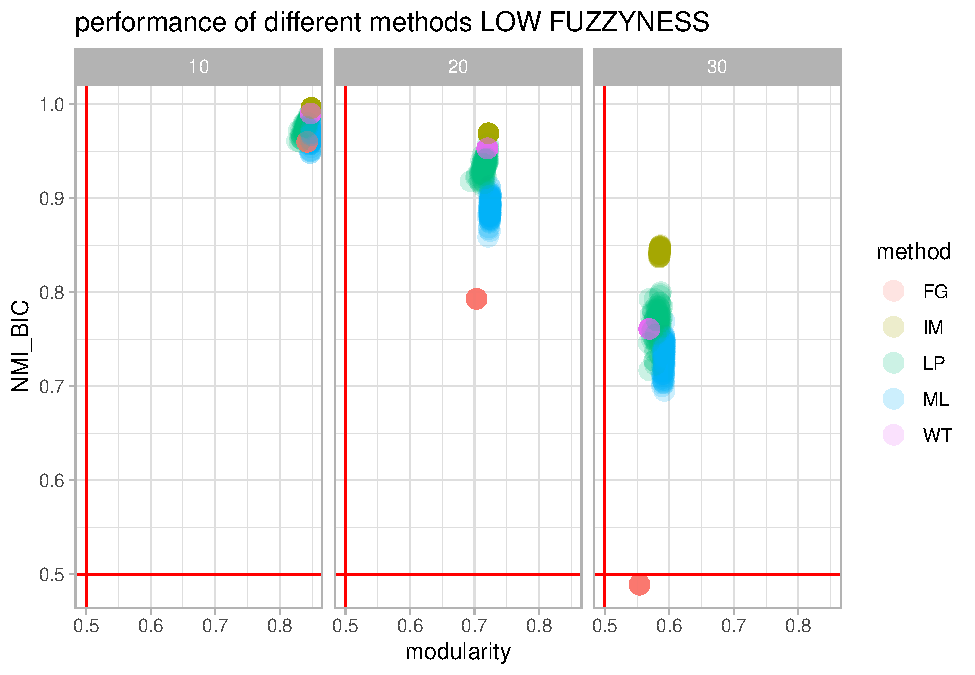
\includegraphics{com_det_algorithms_files/figure-latex/unnamed-chunk-17-1.pdf}

\begin{Shaded}
\begin{Highlighting}[]
\NormalTok{summary\_results }\SpecialCharTok{\%\textgreater{}\%} 
  \FunctionTok{filter}\NormalTok{(mui }\SpecialCharTok{\%in\%} \FunctionTok{c}\NormalTok{(}\DecValTok{35}\NormalTok{,}\DecValTok{40}\NormalTok{)) }\SpecialCharTok{\%\textgreater{}\%} 
  \FunctionTok{ggplot}\NormalTok{(}\FunctionTok{aes}\NormalTok{(}\AttributeTok{x =}\NormalTok{ mod, }\AttributeTok{y =}\NormalTok{ nmi, }\AttributeTok{color =}\NormalTok{ method)) }\SpecialCharTok{+}
  \FunctionTok{geom\_point}\NormalTok{( }\AttributeTok{size =} \DecValTok{4}\NormalTok{, }\AttributeTok{alpha =} \FloatTok{0.5}\NormalTok{) }\SpecialCharTok{+}
  \FunctionTok{geom\_vline}\NormalTok{(}\AttributeTok{xintercept =} \FloatTok{0.5}\NormalTok{, }\AttributeTok{color =} \StringTok{"red"}\NormalTok{)}\SpecialCharTok{+}
  \FunctionTok{geom\_hline}\NormalTok{(}\AttributeTok{yintercept =} \FloatTok{0.5}\NormalTok{, }\AttributeTok{color =} \StringTok{"red"}\NormalTok{)}\SpecialCharTok{+}
  \FunctionTok{labs}\NormalTok{(}\AttributeTok{title =} \StringTok{"performance of different methods TRANSITION "}\NormalTok{, }\AttributeTok{y =} \StringTok{"NMI\_BIC"}\NormalTok{, }\AttributeTok{x =} \StringTok{"modularity"}\NormalTok{) }\SpecialCharTok{+}
  \FunctionTok{theme\_light}\NormalTok{()  }\SpecialCharTok{+} \FunctionTok{facet\_wrap}\NormalTok{(mui }\SpecialCharTok{\textasciitilde{}}\NormalTok{ .)}
\end{Highlighting}
\end{Shaded}

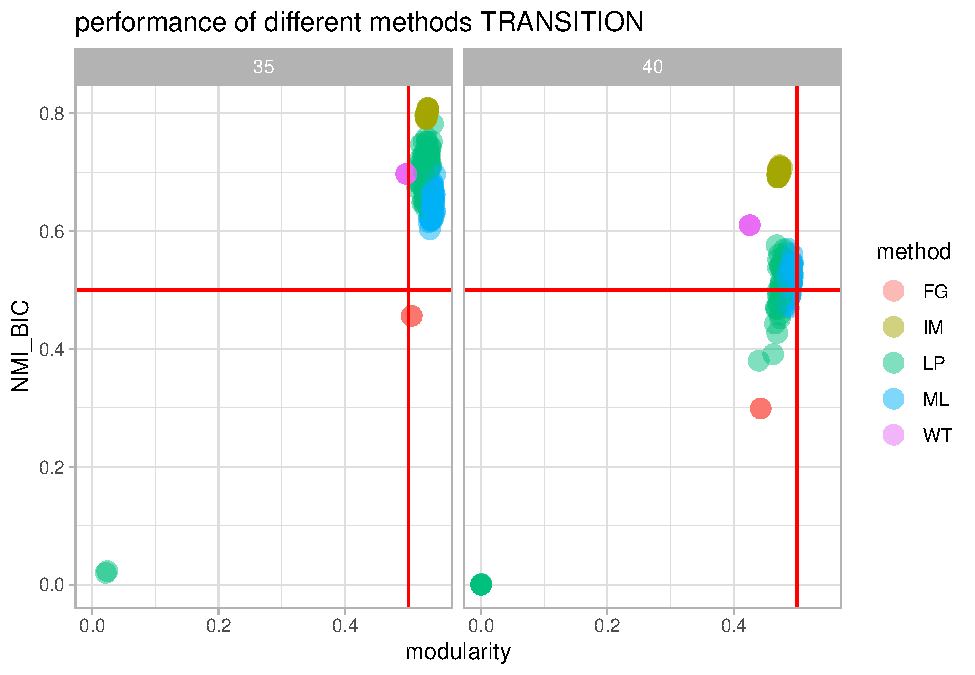
\includegraphics{com_det_algorithms_files/figure-latex/unnamed-chunk-18-1.pdf}

when most methods generate low NMI, we

\begin{Shaded}
\begin{Highlighting}[]
\NormalTok{summary\_results }\SpecialCharTok{\%\textgreater{}\%} 
  \FunctionTok{filter}\NormalTok{(mui }\SpecialCharTok{\%in\%} \FunctionTok{c}\NormalTok{(}\DecValTok{50}\NormalTok{,}\DecValTok{60}\NormalTok{)) }\SpecialCharTok{\%\textgreater{}\%} 
  \FunctionTok{ggplot}\NormalTok{(}\FunctionTok{aes}\NormalTok{(}\AttributeTok{x =}\NormalTok{ mod, }\AttributeTok{y =}\NormalTok{ nmi, }\AttributeTok{color =}\NormalTok{ method)) }\SpecialCharTok{+}
  \FunctionTok{geom\_point}\NormalTok{(}\AttributeTok{size =} \DecValTok{4}\NormalTok{, }\AttributeTok{alpha =} \FloatTok{0.2}\NormalTok{ ) }\SpecialCharTok{+}
  \FunctionTok{geom\_vline}\NormalTok{(}\AttributeTok{xintercept =} \FloatTok{0.5}\NormalTok{, }\AttributeTok{color =} \StringTok{"red"}\NormalTok{)}\SpecialCharTok{+}
  \FunctionTok{geom\_hline}\NormalTok{(}\AttributeTok{yintercept =} \FloatTok{0.5}\NormalTok{, }\AttributeTok{color =} \StringTok{"red"}\NormalTok{)}\SpecialCharTok{+}
  \FunctionTok{labs}\NormalTok{(}\AttributeTok{title =} \StringTok{"performance of different methods HIGH FUZZYNESS "}\NormalTok{, }\AttributeTok{y =} \StringTok{"NMI\_BIC"}\NormalTok{, }\AttributeTok{x =} \StringTok{"modularity"}\NormalTok{) }\SpecialCharTok{+}
  \FunctionTok{theme\_light}\NormalTok{()  }\SpecialCharTok{+} \FunctionTok{facet\_wrap}\NormalTok{(mui }\SpecialCharTok{\textasciitilde{}}\NormalTok{ .)}
\end{Highlighting}
\end{Shaded}

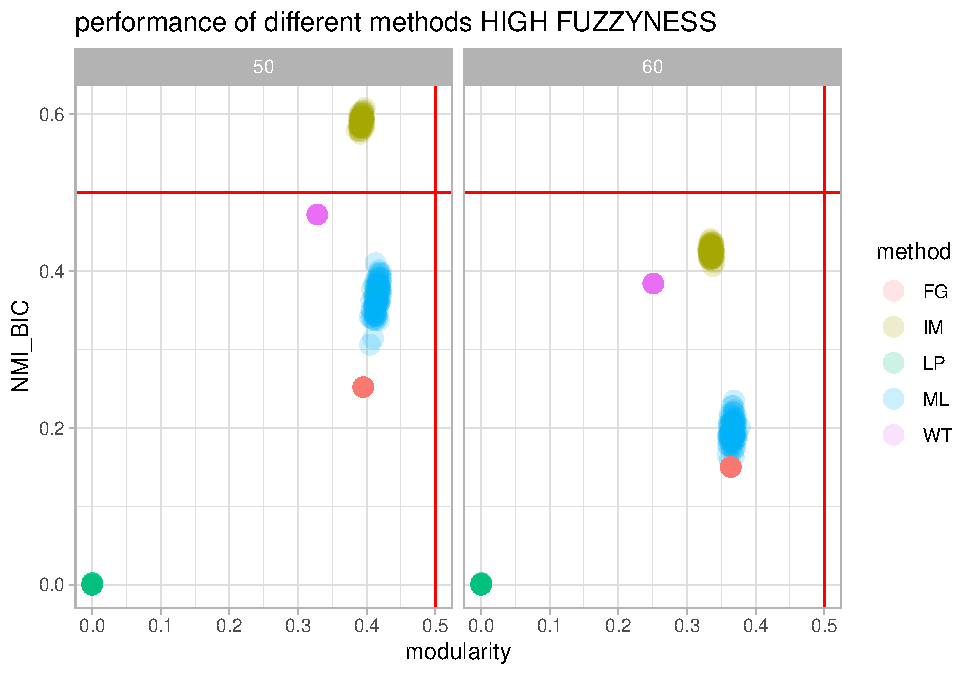
\includegraphics{com_det_algorithms_files/figure-latex/unnamed-chunk-19-1.pdf}

\newpage

\begin{Shaded}
\begin{Highlighting}[]
\NormalTok{summary\_results }\SpecialCharTok{\%\textgreater{}\%} 
  \FunctionTok{filter}\NormalTok{(mui }\SpecialCharTok{\%in\%} \FunctionTok{c}\NormalTok{(}\DecValTok{20}\NormalTok{,}\DecValTok{40}\NormalTok{,}\DecValTok{60}\NormalTok{)) }\SpecialCharTok{\%\textgreater{}\%} 
  \FunctionTok{group\_by}\NormalTok{(method, mui) }\SpecialCharTok{\%\textgreater{}\%} 
    \FunctionTok{summarise}\NormalTok{(}\AttributeTok{mean\_nmi =} \FunctionTok{mean}\NormalTok{(nmi), }\AttributeTok{sd\_nmi =} \FunctionTok{sd}\NormalTok{(nmi), }
              \AttributeTok{mean\_mod =} \FunctionTok{mean}\NormalTok{(mod), }\AttributeTok{sd\_mod =} \FunctionTok{sd}\NormalTok{(mod) ) }\SpecialCharTok{\%\textgreater{}\%}
  \FunctionTok{mutate}\NormalTok{( }\AttributeTok{fuzzyness =} \FunctionTok{case\_when}\NormalTok{(}
\NormalTok{    mui }\SpecialCharTok{==} \DecValTok{20} \SpecialCharTok{\textasciitilde{}} \StringTok{\textquotesingle{}  low fuzzyness\textquotesingle{}}\NormalTok{,}
\NormalTok{    mui }\SpecialCharTok{==} \DecValTok{40} \SpecialCharTok{\textasciitilde{}} \StringTok{\textquotesingle{} transition\textquotesingle{}}\NormalTok{,}
\NormalTok{    mui }\SpecialCharTok{==} \DecValTok{60} \SpecialCharTok{\textasciitilde{}} \StringTok{\textquotesingle{}high fuzzyness\textquotesingle{}}\NormalTok{))}\SpecialCharTok{\%\textgreater{}\%}
  \FunctionTok{ggplot}\NormalTok{(}\FunctionTok{aes}\NormalTok{(}\AttributeTok{x =}\NormalTok{ mean\_mod, }\AttributeTok{y =}\NormalTok{ mean\_nmi, }\AttributeTok{shape =} \FunctionTok{as.factor}\NormalTok{(method), }\AttributeTok{color =}\NormalTok{ fuzzyness)) }\SpecialCharTok{+}
  \FunctionTok{geom\_point}\NormalTok{(}\AttributeTok{size =} \DecValTok{3}\NormalTok{, }\AttributeTok{alpha =} \DecValTok{1}\NormalTok{ ) }\SpecialCharTok{+}
  \FunctionTok{geom\_linerange}\NormalTok{(}\FunctionTok{aes}\NormalTok{(}\AttributeTok{x =}\NormalTok{ mean\_mod, }\AttributeTok{y =}\NormalTok{ mean\_nmi,}\AttributeTok{ymin =}\NormalTok{ mean\_nmi }\SpecialCharTok{{-}}\NormalTok{ sd\_nmi, }\AttributeTok{ymax =}\NormalTok{ mean\_nmi }\SpecialCharTok{+}\NormalTok{ sd\_nmi), }
                 \AttributeTok{linewidth =} \DecValTok{2}\NormalTok{, }\AttributeTok{alpha =} \FloatTok{0.5}\NormalTok{)}\SpecialCharTok{+}
\CommentTok{\#  geom\_linerange(aes(x = mean\_mod, y = mean\_nmi,xmin = mean\_mod {-} sd\_mod, xmax = mean\_mod + sd\_mod), }
\CommentTok{\#                 linewidth = 2, alpha = 0.5)+}
  \FunctionTok{geom\_vline}\NormalTok{(}\AttributeTok{xintercept =} \FloatTok{0.5}\NormalTok{, }\AttributeTok{color =} \StringTok{"red"}\NormalTok{)}\SpecialCharTok{+}
  \FunctionTok{geom\_hline}\NormalTok{(}\AttributeTok{yintercept =} \FloatTok{0.5}\NormalTok{, }\AttributeTok{color =} \StringTok{"red"}\NormalTok{)}\SpecialCharTok{+}
  \FunctionTok{xlim}\NormalTok{(}\DecValTok{0}\NormalTok{,}\DecValTok{1}\NormalTok{)}\SpecialCharTok{+}\CommentTok{\#ylim(0,1)+}
  \FunctionTok{labs}\NormalTok{(}\AttributeTok{title =} \StringTok{"Fuzzyness of communities"}\NormalTok{, }\AttributeTok{x =} \StringTok{"modularity"}\NormalTok{) }\SpecialCharTok{+}
  \FunctionTok{theme\_light}\NormalTok{()  }\CommentTok{\#+ facet\_wrap(fuzzyness \textasciitilde{} .)}
\end{Highlighting}
\end{Shaded}

\begin{verbatim}
## `summarise()` has grouped output by 'method'. You can override using the
## `.groups` argument.
\end{verbatim}

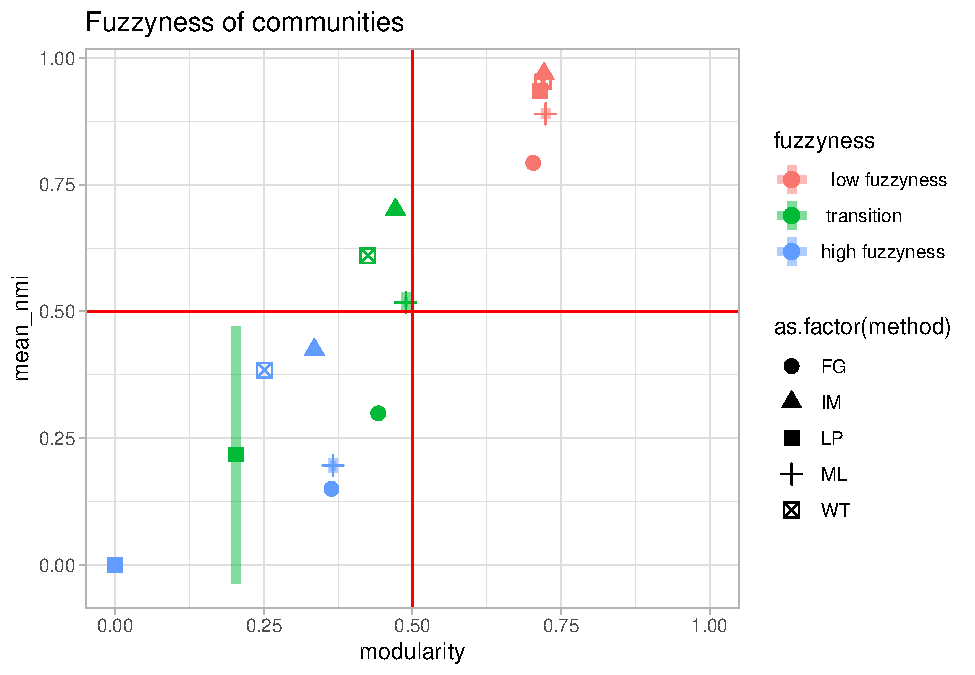
\includegraphics{com_det_algorithms_files/figure-latex/unnamed-chunk-20-1.pdf}

\begin{itemize}
\tightlist
\item
  Low fuzzyness: all methods converge to the same result. Modularity is
  above 0.5
\item
  High fuzzyness: LP collapses to a single community, all other methods
  generate m \textless{} 0.5
\item
  Transition:Other methods diverge: IM, ML and WT are above; FG drops
  below 0.5; LP generates high variance, including collapse.
\end{itemize}

if Low fuzzyness: use LP results if Transition: use IM, ML or WT, and
aggregate small communities if High fuzzyness: use IM or WT, precut,
consensus and aggregate small communities \newpage

\hypertarget{performance-of-different-methods-over-repeated-trials-number-of-communities}{%
\subsection{4.3 performance of different methods over repeated trials:
Number of
Communities}\label{performance-of-different-methods-over-repeated-trials-number-of-communities}}

\begin{Shaded}
\begin{Highlighting}[]
\NormalTok{summary\_results }\SpecialCharTok{\%\textgreater{}\%} 
    \FunctionTok{filter}\NormalTok{(method }\SpecialCharTok{\%in\%} \FunctionTok{c}\NormalTok{( }\StringTok{"FG"}\NormalTok{, }\StringTok{"ML"}\NormalTok{)) }\SpecialCharTok{\%\textgreater{}\%}
  \FunctionTok{ggplot}\NormalTok{(}\FunctionTok{aes}\NormalTok{(}\AttributeTok{x =}\NormalTok{ mui, }\AttributeTok{y =}\NormalTok{ nc)) }\SpecialCharTok{+}
    \FunctionTok{geom\_point}\NormalTok{(}\FunctionTok{aes}\NormalTok{(}\AttributeTok{color =}\NormalTok{ method)) }\SpecialCharTok{+}
    \FunctionTok{labs}\NormalTok{(}\AttributeTok{title =} \StringTok{"Performance of different methods over N trials"}\NormalTok{, }\AttributeTok{y =} \StringTok{"Number of Communitiess"}\NormalTok{, }\AttributeTok{x =} \StringTok{"mu"}\NormalTok{) }\SpecialCharTok{+}
  \FunctionTok{geom\_hline}\NormalTok{(}\AttributeTok{yintercept =} \DecValTok{37}\NormalTok{)}\SpecialCharTok{+}
    \FunctionTok{theme\_light}\NormalTok{() }\SpecialCharTok{+} 
    \FunctionTok{facet\_wrap}\NormalTok{(method }\SpecialCharTok{\textasciitilde{}}\NormalTok{ . )}
\end{Highlighting}
\end{Shaded}

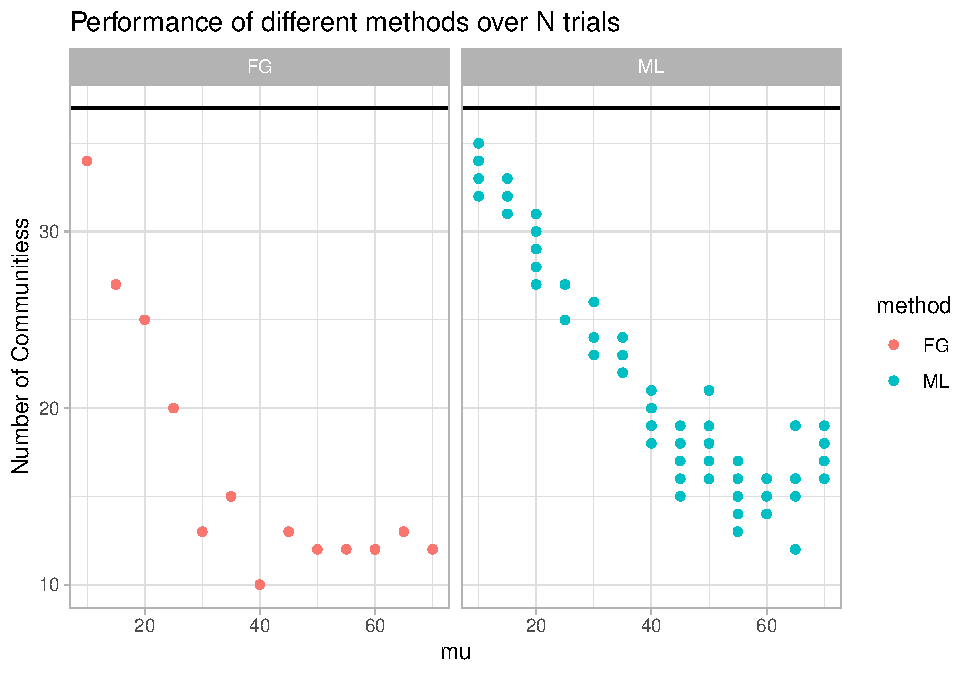
\includegraphics{com_det_algorithms_files/figure-latex/unnamed-chunk-21-1.pdf}

`\texttt{\{r\}\ summary\_results\ \%\textgreater{}\%\ \ \ \ \ \ filter(method\ \%in\%\ c(\ "LP"))\ \%\textgreater{}\%\ \ \ ggplot(aes(x\ =\ mui,\ y\ =\ nc))\ +\ \ \ \ \ geom\_point(aes(color\ =\ method))\ +\ \ \ \ \ labs(title\ =\ "Performance\ of\ different\ methods\ over\ N\ trials",\ y\ =\ "Number\ of\ Communitiess",\ x\ =\ "mu")\ +\ \ \ geom\_hline(yintercept\ =\ 37)+\ \ \ \ \ theme\_light()\ +\ \ \ \ \ \ facet\_wrap(method\ \textasciitilde{}\ .\ )}

\begin{Shaded}
\begin{Highlighting}[]
\NormalTok{summary\_results }\SpecialCharTok{\%\textgreater{}\%} 
    \FunctionTok{filter}\NormalTok{(method }\SpecialCharTok{\%in\%} \FunctionTok{c}\NormalTok{( }\StringTok{"IM"}\NormalTok{,  }\StringTok{"WT"}\NormalTok{)) }\SpecialCharTok{\%\textgreater{}\%}
  \FunctionTok{ggplot}\NormalTok{(}\FunctionTok{aes}\NormalTok{(}\AttributeTok{x =}\NormalTok{ mui, }\AttributeTok{y =}\NormalTok{ nc)) }\SpecialCharTok{+}
    \FunctionTok{geom\_point}\NormalTok{(}\FunctionTok{aes}\NormalTok{(}\AttributeTok{color =}\NormalTok{ method)) }\SpecialCharTok{+}
    \FunctionTok{labs}\NormalTok{(}\AttributeTok{title =} \StringTok{"Performance of different methods over N trials"}\NormalTok{, }\AttributeTok{y =} \StringTok{"Number of Communities"}\NormalTok{, }\AttributeTok{x =} \StringTok{"mu"}\NormalTok{) }\SpecialCharTok{+}
  \FunctionTok{geom\_hline}\NormalTok{(}\AttributeTok{yintercept =} \DecValTok{37}\NormalTok{)}\SpecialCharTok{+}
    \FunctionTok{theme\_light}\NormalTok{() }\SpecialCharTok{+} 
    \FunctionTok{facet\_wrap}\NormalTok{(method }\SpecialCharTok{\textasciitilde{}}\NormalTok{ . , }\AttributeTok{scales =} \StringTok{\textquotesingle{}free\_y\textquotesingle{}}\NormalTok{)}
\end{Highlighting}
\end{Shaded}

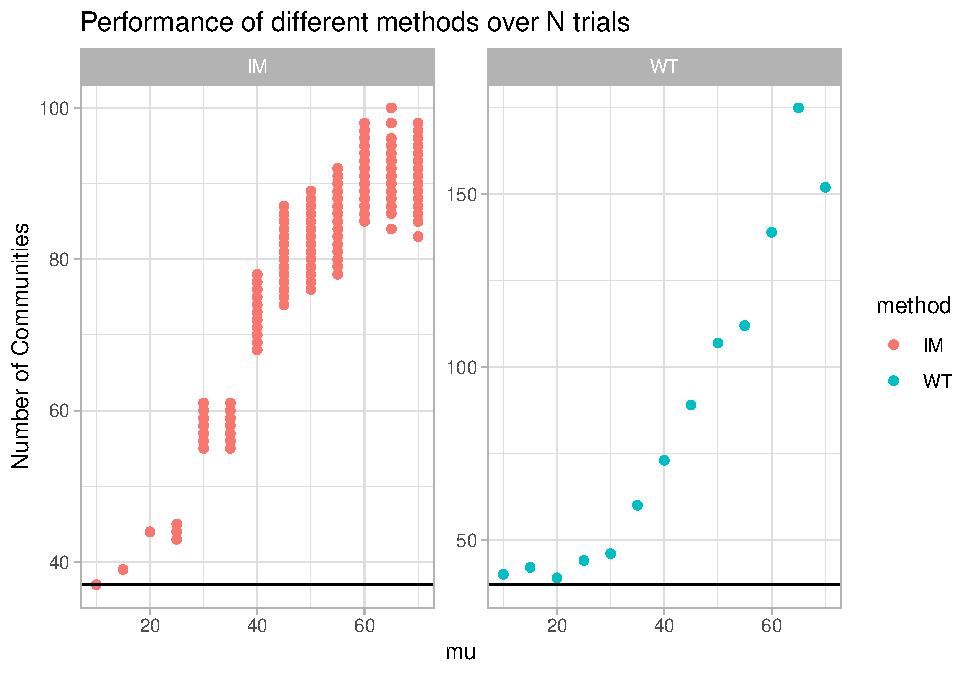
\includegraphics{com_det_algorithms_files/figure-latex/unnamed-chunk-22-1.pdf}

\begin{Shaded}
\begin{Highlighting}[]
\NormalTok{summary\_results }\SpecialCharTok{\%\textgreater{}\%} 
    \FunctionTok{group\_by}\NormalTok{(method, mui) }\SpecialCharTok{\%\textgreater{}\%} 
    \FunctionTok{summarise}\NormalTok{(}\AttributeTok{mean\_nc =} \FunctionTok{mean}\NormalTok{(nc), }\AttributeTok{sd\_nc =} \FunctionTok{sd}\NormalTok{(nc)) }\SpecialCharTok{\%\textgreater{}\%}
    \FunctionTok{ggplot}\NormalTok{(}\FunctionTok{aes}\NormalTok{(}\AttributeTok{x =}\NormalTok{ mui, }\AttributeTok{y =}\NormalTok{ mean\_nc)) }\SpecialCharTok{+}
    \FunctionTok{geom\_point}\NormalTok{(}\FunctionTok{aes}\NormalTok{(}\AttributeTok{color =}\NormalTok{ method)) }\SpecialCharTok{+}
    \FunctionTok{geom\_line}\NormalTok{(}\FunctionTok{aes}\NormalTok{(}\AttributeTok{color =}\NormalTok{ method)) }\SpecialCharTok{+}
    \FunctionTok{geom\_linerange}\NormalTok{(}\FunctionTok{aes}\NormalTok{(}\AttributeTok{ymin =}\NormalTok{mean\_nc}\SpecialCharTok{{-}}\NormalTok{sd\_nc, }\AttributeTok{ymax =}\NormalTok{ mean\_nc }\SpecialCharTok{+}\NormalTok{ sd\_nc, }\AttributeTok{color =}\NormalTok{ method), }\AttributeTok{linewidth =} \DecValTok{2}\NormalTok{, }\AttributeTok{alpha =} \FloatTok{0.5}\NormalTok{)}\SpecialCharTok{+}
    \FunctionTok{geom\_hline}\NormalTok{(}\AttributeTok{yintercept =} \DecValTok{37}\NormalTok{, }\AttributeTok{color =} \StringTok{\textquotesingle{}red\textquotesingle{}}\NormalTok{)}\SpecialCharTok{+}

    \FunctionTok{labs}\NormalTok{(}\AttributeTok{title =} \StringTok{"performance of different methods (Number of Communities)"}\NormalTok{, }\AttributeTok{y =} \StringTok{"number of communities"}\NormalTok{, }\AttributeTok{x =} \StringTok{"mu"}\NormalTok{) }\SpecialCharTok{+}
    \FunctionTok{theme\_light}\NormalTok{()    }
\end{Highlighting}
\end{Shaded}

\begin{verbatim}
## `summarise()` has grouped output by 'method'. You can override using the
## `.groups` argument.
\end{verbatim}

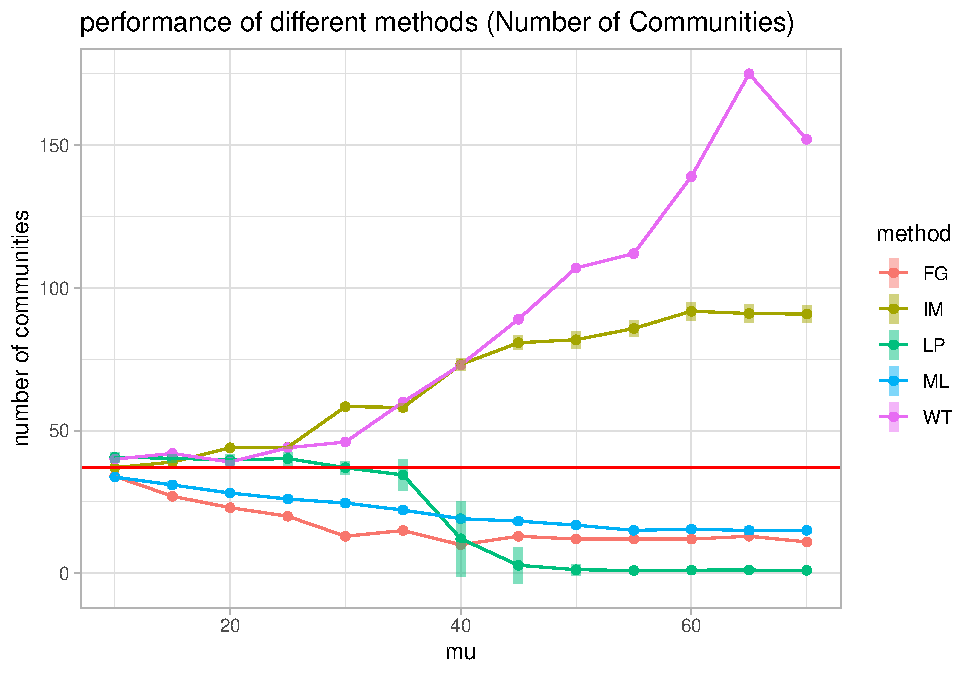
\includegraphics{com_det_algorithms_files/figure-latex/unnamed-chunk-23-1.pdf}

\newpage

\begin{Shaded}
\begin{Highlighting}[]
\NormalTok{summary\_results }\SpecialCharTok{\%\textgreater{}\%} 
  \FunctionTok{filter}\NormalTok{(mui }\SpecialCharTok{\%in\%} \FunctionTok{c}\NormalTok{(}\DecValTok{20}\NormalTok{,}\DecValTok{40}\NormalTok{,}\DecValTok{60}\NormalTok{)) }\SpecialCharTok{\%\textgreater{}\%} 
  \FunctionTok{group\_by}\NormalTok{(method, mui) }\SpecialCharTok{\%\textgreater{}\%} 
    \FunctionTok{summarise}\NormalTok{(}\AttributeTok{mean\_nc =} \FunctionTok{mean}\NormalTok{(nc)}\SpecialCharTok{/}\DecValTok{37}\NormalTok{, }\AttributeTok{sd\_nc =} \FunctionTok{sd}\NormalTok{(nc)}\SpecialCharTok{/}\DecValTok{37}\NormalTok{, }
              \AttributeTok{mean\_mod =} \FunctionTok{mean}\NormalTok{(mod)  ) }\SpecialCharTok{\%\textgreater{}\%}
  \FunctionTok{mutate}\NormalTok{( }\AttributeTok{fuzzyness =} \FunctionTok{case\_when}\NormalTok{(}
\NormalTok{    mui }\SpecialCharTok{==} \DecValTok{20} \SpecialCharTok{\textasciitilde{}} \StringTok{\textquotesingle{}  low fuzzyness\textquotesingle{}}\NormalTok{,}
\NormalTok{    mui }\SpecialCharTok{==} \DecValTok{40} \SpecialCharTok{\textasciitilde{}} \StringTok{\textquotesingle{} transition\textquotesingle{}}\NormalTok{,}
\NormalTok{    mui }\SpecialCharTok{==} \DecValTok{60} \SpecialCharTok{\textasciitilde{}} \StringTok{\textquotesingle{}high fuzzyness\textquotesingle{}}\NormalTok{))}\SpecialCharTok{\%\textgreater{}\%}
  \FunctionTok{ggplot}\NormalTok{(}\FunctionTok{aes}\NormalTok{(}\AttributeTok{x =}\NormalTok{ mean\_mod, }\AttributeTok{y =}\NormalTok{ mean\_nc, }\AttributeTok{shape =} \FunctionTok{as.factor}\NormalTok{(method), }\AttributeTok{color =}\NormalTok{ fuzzyness)) }\SpecialCharTok{+}
  \FunctionTok{geom\_point}\NormalTok{(}\AttributeTok{size =} \DecValTok{3}\NormalTok{, }\AttributeTok{alpha =} \DecValTok{1}\NormalTok{ ) }\SpecialCharTok{+}
  \FunctionTok{geom\_linerange}\NormalTok{(}\FunctionTok{aes}\NormalTok{(}\AttributeTok{x =}\NormalTok{ mean\_mod, }\AttributeTok{y =}\NormalTok{ mean\_nc,}\AttributeTok{ymin =}\NormalTok{ mean\_nc }\SpecialCharTok{{-}}\NormalTok{ sd\_nc, }\AttributeTok{ymax =}\NormalTok{ mean\_nc }\SpecialCharTok{+}\NormalTok{ sd\_nc), }
                 \AttributeTok{linewidth =} \DecValTok{2}\NormalTok{, }\AttributeTok{alpha =} \FloatTok{0.5}\NormalTok{)}\SpecialCharTok{+}
  \FunctionTok{geom\_vline}\NormalTok{(}\AttributeTok{xintercept =} \FloatTok{0.5}\NormalTok{, }\AttributeTok{color =} \StringTok{"red"}\NormalTok{)}\SpecialCharTok{+}
  \FunctionTok{geom\_hline}\NormalTok{(}\AttributeTok{yintercept =} \DecValTok{1}\NormalTok{, }\AttributeTok{color =} \StringTok{"red"}\NormalTok{)}\SpecialCharTok{+}
  \FunctionTok{xlim}\NormalTok{(}\DecValTok{0}\NormalTok{,}\DecValTok{1}\NormalTok{)}\SpecialCharTok{+}\CommentTok{\#ylim(0,1)+}
  \FunctionTok{labs}\NormalTok{(}\AttributeTok{title =} \StringTok{"Fuzzyness of communities"}\NormalTok{, }\AttributeTok{x =} \StringTok{"modularity"}\NormalTok{) }\SpecialCharTok{+}
  \FunctionTok{theme\_light}\NormalTok{() }\CommentTok{\# + facet\_wrap(fuzzyness \textasciitilde{} .)}
\end{Highlighting}
\end{Shaded}

\begin{verbatim}
## `summarise()` has grouped output by 'method'. You can override using the
## `.groups` argument.
\end{verbatim}

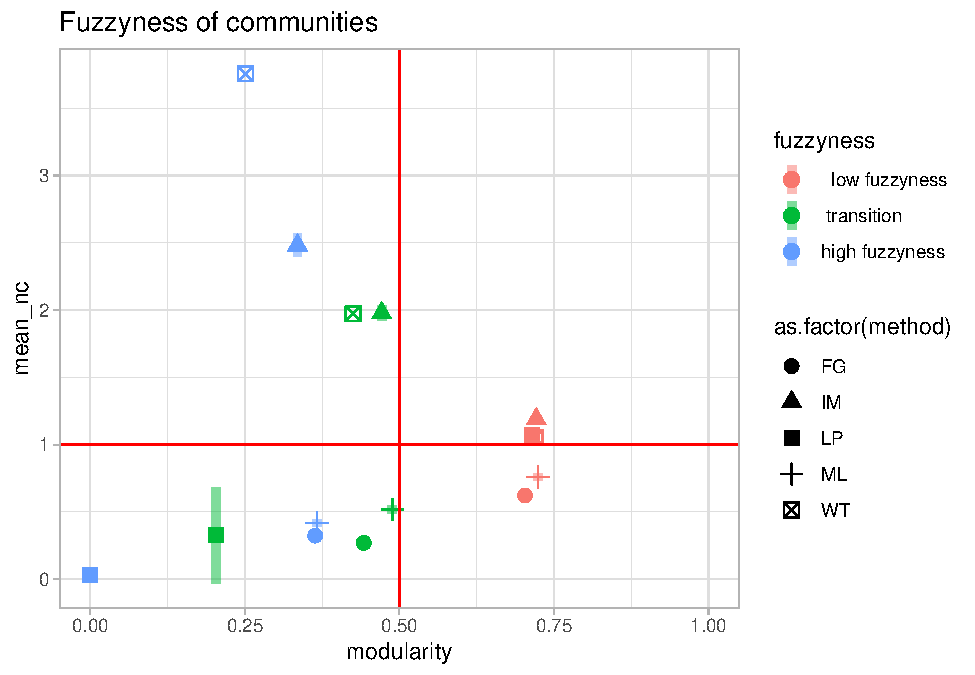
\includegraphics{com_det_algorithms_files/figure-latex/unnamed-chunk-24-1.pdf}

How to improve results if fuzzyness low: use LP or WT if fuzzyness high:
use WT, IM with consensus collapse. or use ML, FG with precut consensus
and collapse if transition: use WT, IM with collapse \newpage

\hypertarget{overal-performance-nmi-nc}{%
\subsection{4.4 overal performance NMI
NC}\label{overal-performance-nmi-nc}}

Performance measured as NMI and NC (improvement: normalize NC/37)

\begin{Shaded}
\begin{Highlighting}[]
\NormalTok{summary\_results }\SpecialCharTok{\%\textgreater{}\%} \FunctionTok{filter}\NormalTok{(mui }\SpecialCharTok{\%in\%}\FunctionTok{c}\NormalTok{(}\DecValTok{20}\NormalTok{,}\DecValTok{40}\NormalTok{,}\DecValTok{60}\NormalTok{)) }\SpecialCharTok{\%\textgreater{}\%}
    \FunctionTok{ggplot}\NormalTok{(}\FunctionTok{aes}\NormalTok{(}\AttributeTok{x =}\NormalTok{ nmi, }\AttributeTok{y =}\NormalTok{ nc}\SpecialCharTok{/}\DecValTok{37}\NormalTok{)) }\SpecialCharTok{+}
    \FunctionTok{geom\_point}\NormalTok{(}\FunctionTok{aes}\NormalTok{(}\AttributeTok{color =}\NormalTok{ method))}\SpecialCharTok{+}
    \FunctionTok{labs}\NormalTok{(}\AttributeTok{title =} \StringTok{"performance of different methods (NMI VS Number of Communities normalized)"}\NormalTok{, }
         \AttributeTok{y =} \StringTok{"number of communities"}\NormalTok{, }\AttributeTok{x =} \StringTok{"NMI"}\NormalTok{) }\SpecialCharTok{+}
    \FunctionTok{geom\_hline}\NormalTok{(}\AttributeTok{yintercept =} \FloatTok{1.0}\NormalTok{, }\AttributeTok{color =} \StringTok{\textquotesingle{}red\textquotesingle{}}\NormalTok{)}\SpecialCharTok{+}
    \FunctionTok{geom\_vline}\NormalTok{(}\AttributeTok{xintercept =} \FloatTok{1.0}\NormalTok{, }\AttributeTok{color =} \StringTok{\textquotesingle{}red\textquotesingle{}}\NormalTok{)}\SpecialCharTok{+}
    \FunctionTok{theme\_light}\NormalTok{()  }\SpecialCharTok{+} \FunctionTok{facet\_wrap}\NormalTok{(mui }\SpecialCharTok{\textasciitilde{}}\NormalTok{ .)}
\end{Highlighting}
\end{Shaded}

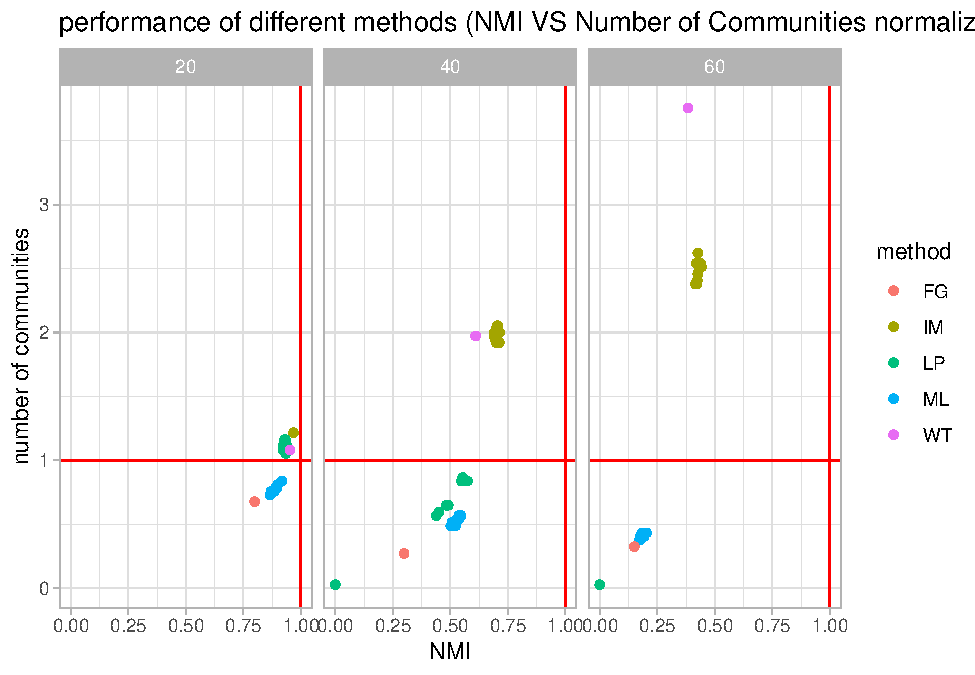
\includegraphics{com_det_algorithms_files/figure-latex/unnamed-chunk-25-1.pdf}

\newpage

\hypertarget{comparing-nmi-with-other-methods-without-built-in-communities}{%
\subsection{comparing NMI with other methods (without Built-in
communities)}\label{comparing-nmi-with-other-methods-without-built-in-communities}}

\begin{Shaded}
\begin{Highlighting}[]
\NormalTok{mts }\OtherTok{\textless{}{-}} \FunctionTok{c}\NormalTok{( }\StringTok{"FG"}\NormalTok{, }\StringTok{"IM"}\NormalTok{, }\StringTok{"LP"}\NormalTok{, }\StringTok{"ML"}\NormalTok{, }\StringTok{"WT"}\NormalTok{)}
\NormalTok{methods }\OtherTok{\textless{}{-}}\NormalTok{ summary\_results}\SpecialCharTok{$}\NormalTok{method}
\NormalTok{nmis }\OtherTok{\textless{}{-}} \FunctionTok{data.frame}\NormalTok{()}
\ControlFlowTok{for}\NormalTok{ (met1 }\ControlFlowTok{in} \DecValTok{1}\SpecialCharTok{:}\FunctionTok{length}\NormalTok{(mts)) \{}
  \ControlFlowTok{for}\NormalTok{ (met2 }\ControlFlowTok{in}\NormalTok{ met1}\SpecialCharTok{:}\FunctionTok{length}\NormalTok{(mts)) \{}
    \ControlFlowTok{if}\NormalTok{ (met1 }\SpecialCharTok{!=}\NormalTok{ met2) \{}
\NormalTok{      mb1 }\OtherTok{\textless{}{-}}\NormalTok{ membership\_matrix[, methods }\SpecialCharTok{==}\NormalTok{ mts[met1]]}
\NormalTok{      mb2 }\OtherTok{\textless{}{-}}\NormalTok{ membership\_matrix[, methods }\SpecialCharTok{==}\NormalTok{ mts[met2]]}
      \ControlFlowTok{for}\NormalTok{ (i }\ControlFlowTok{in} \DecValTok{1}\SpecialCharTok{:}\FunctionTok{ncol}\NormalTok{(mb1)) \{}
        \ControlFlowTok{for}\NormalTok{ (j }\ControlFlowTok{in}\NormalTok{ i}\SpecialCharTok{:}\FunctionTok{ncol}\NormalTok{(mb2)) \{}
          \ControlFlowTok{if}\NormalTok{ (i }\SpecialCharTok{!=}\NormalTok{ j) \{}
\NormalTok{            nmi\_m1\_m2 }\OtherTok{\textless{}{-}}\NormalTok{ aricode}\SpecialCharTok{::}\FunctionTok{NMI}\NormalTok{(mb1[, i], mb2[, j])}
\NormalTok{            nmis }\OtherTok{\textless{}{-}}\FunctionTok{rbind}\NormalTok{(nmis, }\FunctionTok{data.frame}\NormalTok{(methods[met1], methods[met2], met1, met2, nmi\_m1\_m2))}
\NormalTok{          \}}
\NormalTok{        \}}
\NormalTok{      \}}
\NormalTok{    \}}
\NormalTok{  \}}
\NormalTok{\}}
\end{Highlighting}
\end{Shaded}

\begin{Shaded}
\begin{Highlighting}[]
\NormalTok{nmis }\SpecialCharTok{\%\textgreater{}\%} \FunctionTok{ggplot}\NormalTok{()}\SpecialCharTok{+}
  \FunctionTok{geom\_point}\NormalTok{(}\FunctionTok{aes}\NormalTok{(}\AttributeTok{x=}\NormalTok{met1, }\AttributeTok{y =}\NormalTok{ met2, }\AttributeTok{size =}\NormalTok{ (}\DecValTok{100}\SpecialCharTok{*}\NormalTok{nmi\_m1\_m2)}\SpecialCharTok{\^{}}\DecValTok{2}\NormalTok{))  }\SpecialCharTok{+} \FunctionTok{theme\_light}\NormalTok{()}
\end{Highlighting}
\end{Shaded}

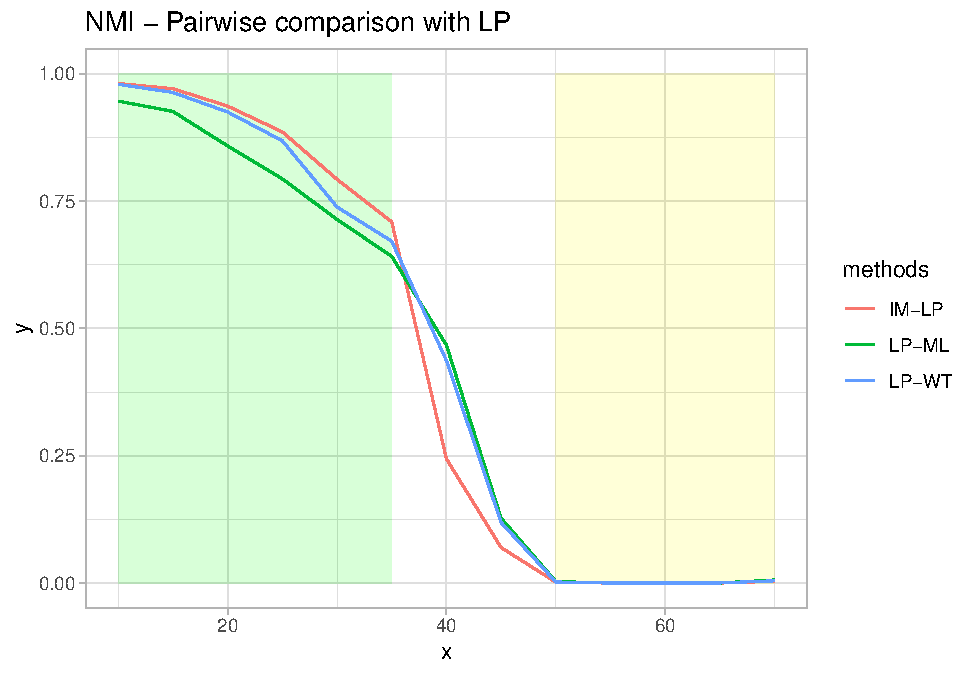
\includegraphics{com_det_algorithms_files/figure-latex/unnamed-chunk-27-1.pdf}

\begin{Shaded}
\begin{Highlighting}[]
\NormalTok{edgelist }\OtherTok{\textless{}{-}}\NormalTok{nmis }\SpecialCharTok{\%\textgreater{}\%} \FunctionTok{mutate}\NormalTok{(}\AttributeTok{weight =}\NormalTok{ nmi\_m1\_m2) }\SpecialCharTok{\%\textgreater{}\%} \FunctionTok{select}\NormalTok{(}\SpecialCharTok{{-}}\NormalTok{met1,}\SpecialCharTok{{-}}\NormalTok{met2,}\SpecialCharTok{{-}}\NormalTok{nmi\_m1\_m2)}
\NormalTok{ggg }\OtherTok{\textless{}{-}} \FunctionTok{graph\_from\_data\_frame}\NormalTok{(edgelist)}
\NormalTok{ggg }\OtherTok{\textless{}{-}} \FunctionTok{as.undirected}\NormalTok{(ggg,}\AttributeTok{mode =} \StringTok{"collapse"}\NormalTok{, }\AttributeTok{edge.attr.comb =} \StringTok{"sum"}\NormalTok{)}
\FunctionTok{plot}\NormalTok{(ggg, }
     \AttributeTok{edge.width=}\FunctionTok{E}\NormalTok{(ggg)}\SpecialCharTok{$}\NormalTok{weight}\SpecialCharTok{*}\FloatTok{0.5}\NormalTok{)}
\end{Highlighting}
\end{Shaded}

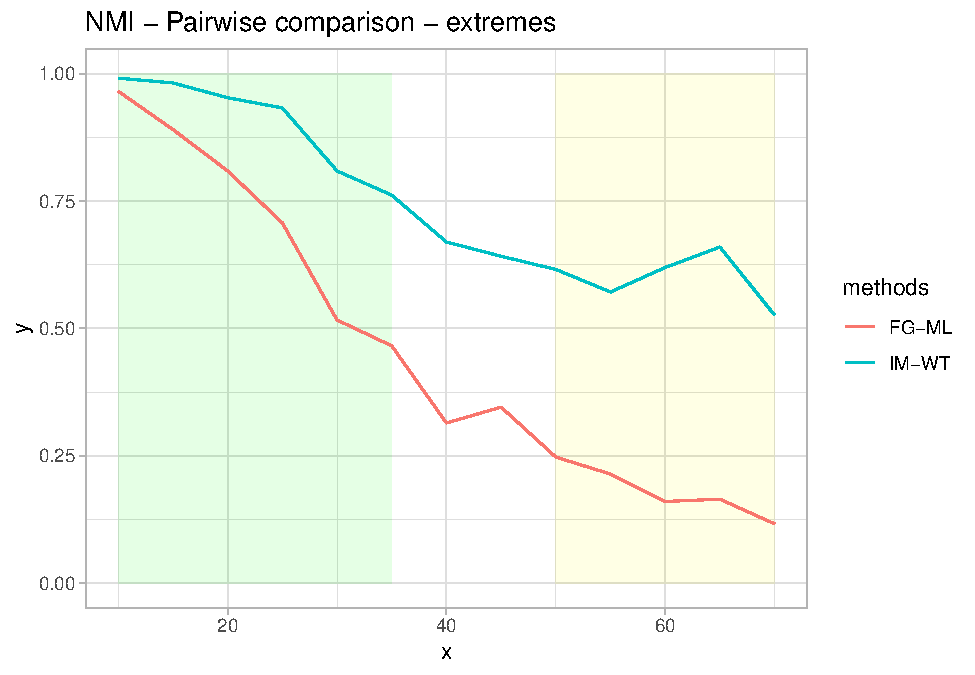
\includegraphics{com_det_algorithms_files/figure-latex/unnamed-chunk-28-1.pdf}

alternative: projection on 1-dimension alternative: take one as a
reference and compare with the others

\newpage

\hypertarget{potential-improvements-by-re-assigning-small-communities-to-community-999}{%
\section{5- potential improvements by re-assigning small communities to
``community
999''}\label{potential-improvements-by-re-assigning-small-communities-to-community-999}}

re-assigning small communities to ``community 999'' can improve NMI and
NC of course only for the methods that overestimate NC

\begin{Shaded}
\begin{Highlighting}[]
\NormalTok{aggregate\_small\_communities }\OtherTok{\textless{}{-}} \ControlFlowTok{function}\NormalTok{(comms, min\_vids, }\AttributeTok{verbose =} \ConstantTok{FALSE}\NormalTok{) \{}
\NormalTok{    comms\_membership }\OtherTok{\textless{}{-}}\NormalTok{ comms}\SpecialCharTok{$}\NormalTok{membership }
\NormalTok{    cs }\OtherTok{\textless{}{-}} \FunctionTok{table}\NormalTok{(comms\_membership)}
    \ControlFlowTok{for}\NormalTok{ (i }\ControlFlowTok{in} \DecValTok{1}\SpecialCharTok{:}\FunctionTok{max}\NormalTok{(comms\_membership)) \{}
        \ControlFlowTok{if}\NormalTok{ (cs[i] }\SpecialCharTok{\textless{}}\NormalTok{ min\_vids) \{}
\NormalTok{            comms\_membership[comms\_membership }\SpecialCharTok{==}\NormalTok{ i] }\OtherTok{\textless{}{-}} \DecValTok{0}
\NormalTok{        \}}
\NormalTok{    \}}
\NormalTok{    comms}\SpecialCharTok{$}\NormalTok{membership }\OtherTok{\textless{}{-}}\NormalTok{ comms\_membership}
    \ControlFlowTok{if}\NormalTok{ (verbose }\SpecialCharTok{==} \ConstantTok{TRUE}\NormalTok{) \{ }
        \FunctionTok{print}\NormalTok{(}\FunctionTok{paste}\NormalTok{(}\StringTok{"Pruning communities below "}\NormalTok{, min\_vids))\}}
    \FunctionTok{return}\NormalTok{(comms)}
\NormalTok{\}}
\end{Highlighting}
\end{Shaded}

Example of pruning

\begin{Shaded}
\begin{Highlighting}[]
\NormalTok{mui }\OtherTok{=} \DecValTok{30}
\NormalTok{method }\OtherTok{=} \StringTok{"IM"}
\NormalTok{g }\OtherTok{\textless{}{-}} \FunctionTok{load\_benchmark\_network}\NormalTok{(}\AttributeTok{mui =}\NormalTok{ mui, }\AttributeTok{path =}\NormalTok{ path, }\AttributeTok{verbose =} \ConstantTok{TRUE}\NormalTok{)}
\end{Highlighting}
\end{Shaded}

\begin{verbatim}
## [1] "Loaded benchmark network ./LFR_graphs/LFR/LFR_benchmark_30.gml"
## [1] "Giant component size : 1000"
## [1] "Built-in communities:  37"
## [1] "Modularity of built-in communities:  0.5778"
\end{verbatim}

\begin{Shaded}
\begin{Highlighting}[]
\NormalTok{comms\_sample }\OtherTok{\textless{}{-}} \FunctionTok{find\_communities}\NormalTok{(g, }\AttributeTok{method =}\NormalTok{ method, }\AttributeTok{verbose =} \ConstantTok{TRUE}\NormalTok{)}
\end{Highlighting}
\end{Shaded}

\begin{verbatim}
## [1] "Community detection with  IM completed."
\end{verbatim}

\begin{Shaded}
\begin{Highlighting}[]
\NormalTok{results }\OtherTok{\textless{}{-}} \FunctionTok{analyse\_communities}\NormalTok{(comms\_sample, mui, }\AttributeTok{verbose =} \ConstantTok{TRUE}\NormalTok{)}
\end{Highlighting}
\end{Shaded}

\begin{verbatim}
## [1] "Communities found:  56"
## [1] "Modularity:  0.5849"
## [1] "Normalized Mutual Information between C.D. method and built-in communities: 0.844"
\end{verbatim}

\begin{Shaded}
\begin{Highlighting}[]
\NormalTok{comms\_aggregated }\OtherTok{\textless{}{-}} \FunctionTok{aggregate\_small\_communities}\NormalTok{(comms\_sample, }\AttributeTok{min\_vids =} \DecValTok{10}\NormalTok{, }\AttributeTok{verbose =} \ConstantTok{TRUE}\NormalTok{)}
\end{Highlighting}
\end{Shaded}

\begin{verbatim}
## [1] "Pruning communities below  10"
\end{verbatim}

\begin{Shaded}
\begin{Highlighting}[]
\NormalTok{results\_aggregated }\OtherTok{\textless{}{-}} \FunctionTok{analyse\_communities}\NormalTok{(comms\_aggregated, mui, }\AttributeTok{verbose =} \ConstantTok{TRUE}\NormalTok{)}
\end{Highlighting}
\end{Shaded}

\begin{verbatim}
## [1] "Communities found:  38"
## [1] "Modularity:  0.5837"
## [1] "Normalized Mutual Information between C.D. method and built-in communities: 0.842"
\end{verbatim}

The number of communities is closer to the built-in value (37), while
there is no relevant change in NMI.

The following shows how pruning impacts NC, usimg method IM and
\(\mu = 0.30\)

\begin{Shaded}
\begin{Highlighting}[]
\NormalTok{mui }\OtherTok{=} \DecValTok{30}
\NormalTok{method }\OtherTok{=} \StringTok{"IM"}
\NormalTok{g }\OtherTok{\textless{}{-}} \FunctionTok{load\_benchmark\_network}\NormalTok{(}\AttributeTok{mui =}\NormalTok{ mui, }\AttributeTok{path =}\NormalTok{ path, }\AttributeTok{verbose =} \ConstantTok{TRUE}\NormalTok{)}
\end{Highlighting}
\end{Shaded}

\begin{verbatim}
## [1] "Loaded benchmark network ./LFR_graphs/LFR/LFR_benchmark_30.gml"
## [1] "Giant component size : 1000"
## [1] "Built-in communities:  37"
## [1] "Modularity of built-in communities:  0.5778"
\end{verbatim}

\begin{Shaded}
\begin{Highlighting}[]
\NormalTok{comms\_sample }\OtherTok{\textless{}{-}} \FunctionTok{find\_communities}\NormalTok{(g, }\AttributeTok{method =}\NormalTok{ method, }\AttributeTok{verbose =} \ConstantTok{TRUE}\NormalTok{)}
\end{Highlighting}
\end{Shaded}

\begin{verbatim}
## [1] "Community detection with  IM completed."
\end{verbatim}

\begin{Shaded}
\begin{Highlighting}[]
\NormalTok{results }\OtherTok{\textless{}{-}} \FunctionTok{analyse\_communities}\NormalTok{(comms\_sample, mui, }\AttributeTok{verbose =} \ConstantTok{TRUE}\NormalTok{)}
\end{Highlighting}
\end{Shaded}

\begin{verbatim}
## [1] "Communities found:  58"
## [1] "Modularity:  0.586"
## [1] "Normalized Mutual Information between C.D. method and built-in communities: 0.845"
\end{verbatim}

\begin{Shaded}
\begin{Highlighting}[]
\ControlFlowTok{for}\NormalTok{ (min\_vids }\ControlFlowTok{in} \DecValTok{1}\SpecialCharTok{:}\DecValTok{12}\NormalTok{)\{}
\NormalTok{    comms\_aggregated }\OtherTok{\textless{}{-}} \FunctionTok{aggregate\_small\_communities}\NormalTok{(comms\_sample, }\AttributeTok{min\_vids =}\NormalTok{ min\_vids, }\AttributeTok{verbose =} \ConstantTok{FALSE}\NormalTok{)}
\NormalTok{    results\_aggregated }\OtherTok{\textless{}{-}} \FunctionTok{analyse\_communities}\NormalTok{(comms\_aggregated, mui , }\AttributeTok{verbose =} \ConstantTok{FALSE}\NormalTok{)}
    \FunctionTok{print}\NormalTok{(}\FunctionTok{paste0}\NormalTok{(}\StringTok{"min\_vids = "}\NormalTok{, min\_vids, }\StringTok{"  NMI = "}\NormalTok{, results\_aggregated}\SpecialCharTok{$}\NormalTok{nmi,}\StringTok{"  NC = "}\NormalTok{,results\_aggregated}\SpecialCharTok{$}\NormalTok{nc ))}
\NormalTok{\}}
\end{Highlighting}
\end{Shaded}

\begin{verbatim}
## [1] "min_vids = 1  NMI = 0.845  NC = 58"
## [1] "min_vids = 2  NMI = 0.845  NC = 58"
## [1] "min_vids = 3  NMI = 0.846  NC = 54"
## [1] "min_vids = 4  NMI = 0.847  NC = 47"
## [1] "min_vids = 5  NMI = 0.847  NC = 47"
## [1] "min_vids = 6  NMI = 0.846  NC = 46"
## [1] "min_vids = 7  NMI = 0.848  NC = 44"
## [1] "min_vids = 8  NMI = 0.853  NC = 40"
## [1] "min_vids = 9  NMI = 0.845  NC = 38"
## [1] "min_vids = 10  NMI = 0.841  NC = 37"
## [1] "min_vids = 11  NMI = 0.841  NC = 37"
## [1] "min_vids = 12  NMI = 0.83  NC = 35"
\end{verbatim}

\newpage

\hypertarget{potential-improvements-by-consensus}{%
\section{6- potential improvements by
consensus}\label{potential-improvements-by-consensus}}

Consensus helps improving performance (applicable to methods that
underestimate NV, as it generates a number of small communities, AND
have some intrinsic variability of results)

\begin{Shaded}
\begin{Highlighting}[]
\NormalTok{normalized\_co\_occurrence }\OtherTok{\textless{}{-}} \ControlFlowTok{function}\NormalTok{(all\_clusters)\{}
\NormalTok{  n\_trials }\OtherTok{\textless{}{-}} \FunctionTok{ncol}\NormalTok{(all\_clusters)}
\NormalTok{    x }\OtherTok{\textless{}{-}} \FunctionTok{matrix}\NormalTok{(}\DecValTok{0}\NormalTok{,}\AttributeTok{nrow =} \FunctionTok{nrow}\NormalTok{(all\_clusters),}\AttributeTok{ncol =} \FunctionTok{nrow}\NormalTok{(all\_clusters))}
    \FunctionTok{colnames}\NormalTok{(x) }\OtherTok{\textless{}{-}} \FunctionTok{V}\NormalTok{(g)}\SpecialCharTok{$}\NormalTok{name}
    \FunctionTok{rownames}\NormalTok{(x) }\OtherTok{\textless{}{-}} \FunctionTok{V}\NormalTok{(g)}\SpecialCharTok{$}\NormalTok{name}
    \ControlFlowTok{for}\NormalTok{ (i }\ControlFlowTok{in}\NormalTok{ (}\DecValTok{1}\SpecialCharTok{:}\NormalTok{n\_trials)) \{}
\NormalTok{        nclusters }\OtherTok{\textless{}{-}} \FunctionTok{max}\NormalTok{(all\_clusters[, i])}
        \ControlFlowTok{for}\NormalTok{ (k }\ControlFlowTok{in} \DecValTok{1}\SpecialCharTok{:}\NormalTok{nclusters) \{}
\NormalTok{            samecluster }\OtherTok{\textless{}{-}}\NormalTok{ (}\FunctionTok{which}\NormalTok{(all\_clusters[, i] }\SpecialCharTok{==}\NormalTok{ k))}
\NormalTok{            nc }\OtherTok{\textless{}{-}} \FunctionTok{length}\NormalTok{(samecluster)}
            \ControlFlowTok{for}\NormalTok{ (t }\ControlFlowTok{in} \DecValTok{1}\SpecialCharTok{:}\NormalTok{nc) \{}
                \ControlFlowTok{for}\NormalTok{ (j }\ControlFlowTok{in} \DecValTok{1}\SpecialCharTok{:}\NormalTok{nc) \{}
\NormalTok{                    x[samecluster[j], samecluster[t]] }\OtherTok{\textless{}{-}}
\NormalTok{                        x[samecluster[j], samecluster[t]] }\SpecialCharTok{+} \DecValTok{1}
\NormalTok{                \}}
\NormalTok{            \}}
\NormalTok{        \}}
\NormalTok{    \}}
    \FunctionTok{return}\NormalTok{ (x}\SpecialCharTok{/} \FunctionTok{ncol}\NormalTok{(all\_clusters))}
\NormalTok{\}}
\end{Highlighting}
\end{Shaded}

\newpage

\begin{Shaded}
\begin{Highlighting}[]
\NormalTok{consensus }\OtherTok{\textless{}{-}}\ControlFlowTok{function}\NormalTok{(all\_clusters, }\AttributeTok{min\_p =} \FloatTok{0.01}\NormalTok{,}\AttributeTok{min\_vids =} \DecValTok{1}\NormalTok{,}\AttributeTok{verbose =} \ConstantTok{FALSE}\NormalTok{) \{}
\NormalTok{    remaining }\OtherTok{\textless{}{-}}\FunctionTok{normalized\_co\_occurrence}\NormalTok{(all\_clusters)}
\NormalTok{    v.processed }\OtherTok{\textless{}{-}} \DecValTok{0}
\NormalTok{    current.cluster }\OtherTok{=} \DecValTok{0}
\NormalTok{    ccs }\OtherTok{\textless{}{-}} \FunctionTok{data.frame}\NormalTok{(}\AttributeTok{name =} \FunctionTok{V}\NormalTok{(g)}\SpecialCharTok{$}\NormalTok{name)}
\NormalTok{    ccs}\SpecialCharTok{$}\NormalTok{mbshp }\OtherTok{=} \FunctionTok{rep}\NormalTok{(}\DecValTok{0}\NormalTok{, }\FunctionTok{nrow}\NormalTok{(ccs))}
\NormalTok{    ccs}\SpecialCharTok{$}\NormalTok{prob }\OtherTok{=} \FunctionTok{apply}\NormalTok{(remaining, }\DecValTok{1}\NormalTok{, max)}
\NormalTok{    more\_clusters\_to\_process }\OtherTok{=} \ConstantTok{TRUE}
    \ControlFlowTok{while}\NormalTok{ (more\_clusters\_to\_process) \{}
\NormalTok{      cluster\_ii\_members }\OtherTok{\textless{}{-}} \FunctionTok{which}\NormalTok{(remaining[}\DecValTok{1}\NormalTok{, ] }\SpecialCharTok{\textgreater{}}\NormalTok{ min\_p)}
\NormalTok{      v.processed }\OtherTok{\textless{}{-}}\NormalTok{ v.processed }\SpecialCharTok{+} \FunctionTok{length}\NormalTok{(cluster\_ii\_members)}
      \ControlFlowTok{if}\NormalTok{ (verbose }\SpecialCharTok{==} \ConstantTok{TRUE}\NormalTok{) \{}
        \FunctionTok{print}\NormalTok{(}\FunctionTok{paste}\NormalTok{(}\StringTok{"start While loop with v to process = "}\NormalTok{,}\FunctionTok{dim}\NormalTok{(remaining)[}\DecValTok{1}\NormalTok{],v.processed))}
\NormalTok{      \}}
\NormalTok{      selected }\OtherTok{\textless{}{-}}\NormalTok{remaining[cluster\_ii\_members, cluster\_ii\_members]}
      \ControlFlowTok{if}\NormalTok{ (}\FunctionTok{is.matrix}\NormalTok{(selected)) \{}
        \FunctionTok{diag}\NormalTok{(selected) }\OtherTok{\textless{}{-}} \DecValTok{0} \CommentTok{\# diagonal elements are not relevant}
        \ControlFlowTok{if}\NormalTok{ ( (}\FunctionTok{length}\NormalTok{(cluster\_ii\_members) }\SpecialCharTok{\textgreater{}}\NormalTok{ min\_vids) }\SpecialCharTok{==} \ConstantTok{TRUE}\NormalTok{) \{}
\NormalTok{          current.cluster }\OtherTok{\textless{}{-}}\NormalTok{ current.cluster }\SpecialCharTok{+} \DecValTok{1}
          \ControlFlowTok{if}\NormalTok{ (verbose }\SpecialCharTok{==} \ConstantTok{TRUE}\NormalTok{) \{}
            \FunctionTok{print}\NormalTok{(}\FunctionTok{paste}\NormalTok{(}\StringTok{"community"}\NormalTok{,current.cluster,}\FunctionTok{max}\NormalTok{(selected),}\FunctionTok{length}\NormalTok{(cluster\_ii\_members)))}
\NormalTok{          \}}
          \ControlFlowTok{for}\NormalTok{ (j }\ControlFlowTok{in} \DecValTok{1}\SpecialCharTok{:}\FunctionTok{nrow}\NormalTok{(selected)) \{}
\NormalTok{            nn }\OtherTok{\textless{}{-}} \FunctionTok{names}\NormalTok{(selected[}\DecValTok{1}\NormalTok{, ])[j]}
            \ControlFlowTok{if}\NormalTok{ (verbose }\SpecialCharTok{==} \ConstantTok{TRUE}\NormalTok{)  \{}
              \FunctionTok{print}\NormalTok{(}\FunctionTok{paste}\NormalTok{(}\StringTok{"Adding"}\NormalTok{,nn,}\StringTok{"to comm"}\NormalTok{,current.cluster))}
\NormalTok{            \}}
\NormalTok{            ccs}\SpecialCharTok{$}\NormalTok{mbshp[ccs}\SpecialCharTok{$}\NormalTok{name }\SpecialCharTok{==}\NormalTok{ nn] }\OtherTok{\textless{}{-}}\NormalTok{ current.cluster}
\NormalTok{            ccs}\SpecialCharTok{$}\NormalTok{prob[ccs}\SpecialCharTok{$}\NormalTok{name }\SpecialCharTok{==}\NormalTok{ nn] }\OtherTok{\textless{}{-}} \FunctionTok{max}\NormalTok{(selected[j, ])}
\NormalTok{          \}}
\NormalTok{        \} }\ControlFlowTok{else}\NormalTok{ \{}
          \ControlFlowTok{if}\NormalTok{ (verbose }\SpecialCharTok{==} \ConstantTok{TRUE}\NormalTok{)  \{}
            \FunctionTok{print}\NormalTok{(}\FunctionTok{paste}\NormalTok{(}\StringTok{"community zero"}\NormalTok{,}\FunctionTok{max}\NormalTok{(selected),}\FunctionTok{length}\NormalTok{(cluster\_ii\_members)))}
\NormalTok{          \}}
          \ControlFlowTok{for}\NormalTok{ (j }\ControlFlowTok{in} \DecValTok{1}\SpecialCharTok{:}\FunctionTok{nrow}\NormalTok{(selected)) \{}
\NormalTok{            nn }\OtherTok{\textless{}{-}} \FunctionTok{names}\NormalTok{(selected[}\DecValTok{1}\NormalTok{, ])[j]}
\NormalTok{            ccs}\SpecialCharTok{$}\NormalTok{mbshp[ccs}\SpecialCharTok{$}\NormalTok{name }\SpecialCharTok{==}\NormalTok{ nn] }\OtherTok{\textless{}{-}}  \DecValTok{0}
\NormalTok{            ccs}\SpecialCharTok{$}\NormalTok{prob[ccs}\SpecialCharTok{$}\NormalTok{name }\SpecialCharTok{==}\NormalTok{ nn] }\OtherTok{\textless{}{-}}  \FunctionTok{max}\NormalTok{(selected)}
\NormalTok{          \}}
\NormalTok{        \}}
\NormalTok{      \}}
\NormalTok{      tmp }\OtherTok{\textless{}{-}}\NormalTok{remaining[}\SpecialCharTok{{-}}\NormalTok{cluster\_ii\_members,}\SpecialCharTok{{-}}\NormalTok{cluster\_ii\_members]}
      \ControlFlowTok{if}\NormalTok{ (}\FunctionTok{is.matrix}\NormalTok{(tmp)) \{}
        \ControlFlowTok{if}\NormalTok{ (}\FunctionTok{dim}\NormalTok{(tmp)[}\DecValTok{1}\NormalTok{] }\SpecialCharTok{\textless{}=} \DecValTok{1}\NormalTok{) \{}
\NormalTok{          more\_clusters\_to\_process }\OtherTok{\textless{}{-}} \ConstantTok{FALSE}
\NormalTok{        \}}
\NormalTok{        remaining }\OtherTok{\textless{}{-}}\NormalTok{ tmp}
\NormalTok{      \} }\ControlFlowTok{else}\NormalTok{ \{}
\NormalTok{        more\_clusters\_to\_process }\OtherTok{\textless{}{-}} \ConstantTok{FALSE}
\NormalTok{      \}}
\NormalTok{    \}}
    \FunctionTok{return}\NormalTok{(ccs)}
\NormalTok{  \}}
\end{Highlighting}
\end{Shaded}

\newpage

Examples

\begin{Shaded}
\begin{Highlighting}[]
\NormalTok{n\_trials }\OtherTok{\textless{}{-}} \DecValTok{100}
\NormalTok{method }\OtherTok{\textless{}{-}} \StringTok{\textquotesingle{}ML\textquotesingle{}}
\NormalTok{all\_clusters }\OtherTok{\textless{}{-}} \FunctionTok{c}\NormalTok{()}
\NormalTok{mui }\OtherTok{=} \DecValTok{20}
\NormalTok{g }\OtherTok{\textless{}{-}} \FunctionTok{load\_benchmark\_network}\NormalTok{(}\AttributeTok{mui =}\NormalTok{ mui, }\AttributeTok{path =}\NormalTok{ path, }\AttributeTok{verbose =} \ConstantTok{TRUE}\NormalTok{)}
\end{Highlighting}
\end{Shaded}

\begin{verbatim}
## [1] "Loaded benchmark network ./LFR_graphs/LFR/LFR_benchmark_20.gml"
## [1] "Giant component size : 999"
## [1] "Built-in communities:  37"
## [1] "Modularity of built-in communities:  0.7229"
\end{verbatim}

\begin{Shaded}
\begin{Highlighting}[]
\ControlFlowTok{for}\NormalTok{ (i }\ControlFlowTok{in} \DecValTok{1}\SpecialCharTok{:}\NormalTok{n\_trials)\{}
\NormalTok{    comms\_i }\OtherTok{\textless{}{-}} \FunctionTok{find\_communities}\NormalTok{(g, }\AttributeTok{method =}\NormalTok{ method)}
\NormalTok{    all\_clusters }\OtherTok{\textless{}{-}} \FunctionTok{cbind}\NormalTok{(all\_clusters, comms\_i}\SpecialCharTok{$}\NormalTok{membership)}
\NormalTok{\}}
\CommentTok{\#print("Results of last single trial")}
\NormalTok{results }\OtherTok{\textless{}{-}} \FunctionTok{analyse\_communities}\NormalTok{(comms\_i, mui, }\AttributeTok{verbose =} \ConstantTok{TRUE}\NormalTok{)}
\end{Highlighting}
\end{Shaded}

\begin{verbatim}
## [1] "Communities found:  28"
## [1] "Modularity:  0.7249"
## [1] "Normalized Mutual Information between C.D. method and built-in communities: 0.886"
\end{verbatim}

\begin{Shaded}
\begin{Highlighting}[]
\CommentTok{\#print("Results of consensus")}
\NormalTok{cons\_results }\OtherTok{\textless{}{-}} \FunctionTok{consensus}\NormalTok{(all\_clusters, }\AttributeTok{min\_p =} \FloatTok{0.5}\NormalTok{)}
\NormalTok{cons\_communities }\OtherTok{\textless{}{-}} \FunctionTok{make\_clusters}\NormalTok{(g, }\FunctionTok{array}\NormalTok{(cons\_results}\SpecialCharTok{$}\NormalTok{mbshp}\SpecialCharTok{+}\DecValTok{1}\NormalTok{))}
\NormalTok{cons\_communities}\SpecialCharTok{$}\NormalTok{algorithm }\OtherTok{\textless{}{-}} \FunctionTok{paste0}\NormalTok{(method,}\StringTok{"\_cons"}\NormalTok{)}
\NormalTok{cons\_communities}\SpecialCharTok{$}\NormalTok{rm }\OtherTok{\textless{}{-}}\NormalTok{cons\_results}\SpecialCharTok{$}\NormalTok{prob}
\FunctionTok{V}\NormalTok{(g)}\SpecialCharTok{$}\NormalTok{rm }\OtherTok{\textless{}{-}}\NormalTok{ cons\_results}\SpecialCharTok{$}\NormalTok{prob}

\NormalTok{results\_cons }\OtherTok{\textless{}{-}} \FunctionTok{analyse\_communities}\NormalTok{(cons\_communities, mui, }\AttributeTok{verbose =} \ConstantTok{TRUE}\NormalTok{)}
\end{Highlighting}
\end{Shaded}

\begin{verbatim}
## [1] "Communities found:  33"
## [1] "Modularity:  0.7243"
## [1] "Normalized Mutual Information between C.D. method and built-in communities: 0.922"
\end{verbatim}

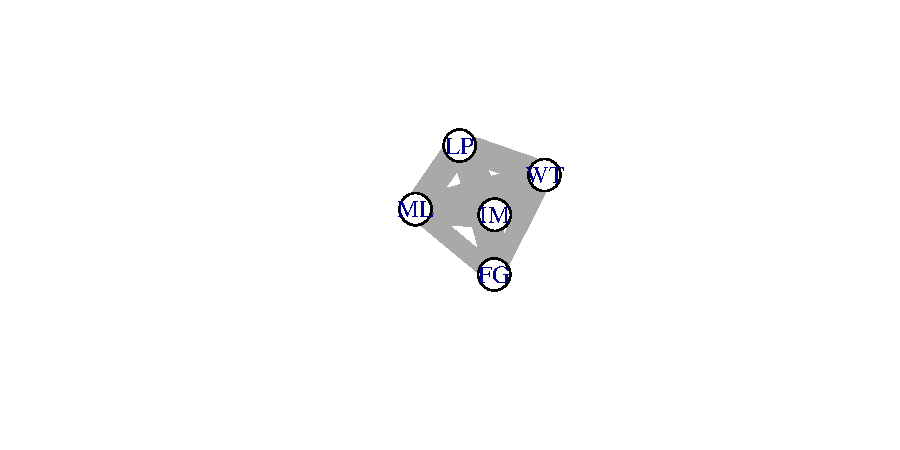
\includegraphics{com_det_algorithms_files/figure-latex/unnamed-chunk-31-1.pdf}

\begin{Shaded}
\begin{Highlighting}[]
\FunctionTok{hist}\NormalTok{(cons\_results}\SpecialCharTok{$}\NormalTok{prob)}
\end{Highlighting}
\end{Shaded}

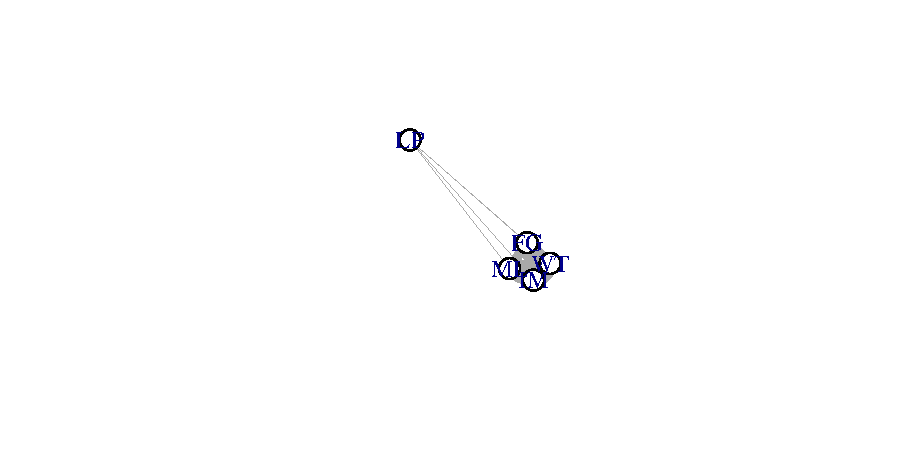
\includegraphics{com_det_algorithms_files/figure-latex/unnamed-chunk-32-1.pdf}

\newpage

\hypertarget{potential-improvements-by-pre-cut}{%
\section{7- potential improvements by
pre-cut}\label{potential-improvements-by-pre-cut}}

improving performance by pre-cut on methods that underestimate NC

\begin{Shaded}
\begin{Highlighting}[]
\NormalTok{pre\_cut\_network }\OtherTok{\textless{}{-}} \ControlFlowTok{function}\NormalTok{(g,}
                            \AttributeTok{alpha =} \FloatTok{0.05}\NormalTok{,}
                            \AttributeTok{epsilon =} \DecValTok{1} \SpecialCharTok{/} \DecValTok{1000}\NormalTok{) \{}
\NormalTok{  g\_pre\_cut }\OtherTok{\textless{}{-}}\NormalTok{ g}
\NormalTok{  n\_items }\OtherTok{\textless{}{-}} \FunctionTok{length}\NormalTok{(}\FunctionTok{E}\NormalTok{(g\_pre\_cut))}
\NormalTok{  n\_null }\OtherTok{\textless{}{-}} \FunctionTok{as.integer}\NormalTok{(alpha }\SpecialCharTok{*}\NormalTok{ n\_items)}
\NormalTok{  applied\_weights }\OtherTok{\textless{}{-}} \FunctionTok{E}\NormalTok{(g\_pre\_cut)}\SpecialCharTok{$}\NormalTok{ww}
\NormalTok{  applied\_weights[}\FunctionTok{sample}\NormalTok{(n\_items, n\_null)] }\OtherTok{\textless{}{-}}\NormalTok{ epsilon}
  \FunctionTok{E}\NormalTok{(g\_pre\_cut)}\SpecialCharTok{$}\NormalTok{weight }\OtherTok{\textless{}{-}}\NormalTok{ applied\_weights}
  \FunctionTok{return}\NormalTok{(g\_pre\_cut)}
\NormalTok{\}}
\end{Highlighting}
\end{Shaded}

\begin{Shaded}
\begin{Highlighting}[]
\NormalTok{g }\OtherTok{\textless{}{-}} \FunctionTok{load\_benchmark\_network}\NormalTok{(}\AttributeTok{mui =} \DecValTok{50}\NormalTok{, }\AttributeTok{path =}\NormalTok{ path, }\AttributeTok{verbose =} \ConstantTok{TRUE}\NormalTok{)}
\end{Highlighting}
\end{Shaded}

\begin{verbatim}
## [1] "Loaded benchmark network ./LFR_graphs/LFR/LFR_benchmark_50.gml"
## [1] "Giant component size : 999"
## [1] "Built-in communities:  37"
## [1] "Modularity of built-in communities:  0.3639"
\end{verbatim}

\begin{Shaded}
\begin{Highlighting}[]
\NormalTok{gp }\OtherTok{\textless{}{-}} \FunctionTok{pre\_cut\_network}\NormalTok{(g,  }\AttributeTok{alpha =} \FloatTok{0.30}\NormalTok{, }\AttributeTok{epsilon =} \DecValTok{1}\SpecialCharTok{/}\DecValTok{1000}\NormalTok{)}
\FunctionTok{hist}\NormalTok{(}\FunctionTok{strength}\NormalTok{(g))}
\end{Highlighting}
\end{Shaded}

\includegraphics{com_det_algorithms_files/figure-latex/unnamed-chunk-34-1.pdf}

\begin{Shaded}
\begin{Highlighting}[]
\FunctionTok{hist}\NormalTok{(}\FunctionTok{strength}\NormalTok{(gp))}
\end{Highlighting}
\end{Shaded}

\includegraphics{com_det_algorithms_files/figure-latex/unnamed-chunk-34-2.pdf}

\newpage

\begin{Shaded}
\begin{Highlighting}[]
\NormalTok{n\_trials }\OtherTok{\textless{}{-}} \DecValTok{100}
\NormalTok{method }\OtherTok{\textless{}{-}} \StringTok{\textquotesingle{}LV\textquotesingle{}}
\NormalTok{all\_clusters }\OtherTok{\textless{}{-}} \FunctionTok{c}\NormalTok{()}
\NormalTok{mui }\OtherTok{=} \DecValTok{30}
\NormalTok{g }\OtherTok{\textless{}{-}} \FunctionTok{load\_benchmark\_network}\NormalTok{(}\AttributeTok{mui =}\NormalTok{ mui, }\AttributeTok{path =}\NormalTok{ path, }\AttributeTok{verbose =} \ConstantTok{TRUE}\NormalTok{)}
\end{Highlighting}
\end{Shaded}

\begin{verbatim}
## [1] "Loaded benchmark network ./LFR_graphs/LFR/LFR_benchmark_30.gml"
## [1] "Giant component size : 1000"
## [1] "Built-in communities:  37"
## [1] "Modularity of built-in communities:  0.5778"
\end{verbatim}

\begin{Shaded}
\begin{Highlighting}[]
\ControlFlowTok{for}\NormalTok{ (i }\ControlFlowTok{in} \DecValTok{1}\SpecialCharTok{:}\NormalTok{n\_trials)\{}
\NormalTok{  gp }\OtherTok{\textless{}{-}} \FunctionTok{pre\_cut\_network}\NormalTok{(g,  }\AttributeTok{alpha =} \FloatTok{0.10}\NormalTok{, }\AttributeTok{epsilon =} \DecValTok{1}\SpecialCharTok{/}\DecValTok{1000}\NormalTok{)}
\NormalTok{  comms\_i }\OtherTok{\textless{}{-}} \FunctionTok{find\_communities}\NormalTok{(gp, }\AttributeTok{method =}\NormalTok{ method)}
\NormalTok{  all\_clusters }\OtherTok{\textless{}{-}} \FunctionTok{cbind}\NormalTok{(all\_clusters, comms\_i}\SpecialCharTok{$}\NormalTok{membership)}
\NormalTok{\}}
\CommentTok{\#print("Results of last single trial")}
\NormalTok{results }\OtherTok{\textless{}{-}} \FunctionTok{analyse\_communities}\NormalTok{(comms\_i, mui, }\AttributeTok{verbose =} \ConstantTok{TRUE}\NormalTok{)}
\end{Highlighting}
\end{Shaded}

\begin{verbatim}
## [1] "Communities found:  24"
## [1] "Modularity:  0.5845"
## [1] "Normalized Mutual Information between C.D. method and built-in communities: 0.7"
\end{verbatim}

\begin{Shaded}
\begin{Highlighting}[]
\CommentTok{\#print("Results of consensus")}
\NormalTok{cons\_results }\OtherTok{\textless{}{-}} \FunctionTok{consensus}\NormalTok{(all\_clusters, }\AttributeTok{min\_p =} \FloatTok{0.5}\NormalTok{)}
\NormalTok{cons\_communities }\OtherTok{\textless{}{-}} \FunctionTok{make\_clusters}\NormalTok{(gp, }\FunctionTok{array}\NormalTok{(cons\_results}\SpecialCharTok{$}\NormalTok{mbshp}\SpecialCharTok{+}\DecValTok{1}\NormalTok{))}
\NormalTok{cons\_communities}\SpecialCharTok{$}\NormalTok{algorithm }\OtherTok{\textless{}{-}} \FunctionTok{paste0}\NormalTok{(method,}\StringTok{"\_cons"}\NormalTok{)}
\NormalTok{cons\_communities}\SpecialCharTok{$}\NormalTok{rm }\OtherTok{\textless{}{-}}\NormalTok{cons\_results}\SpecialCharTok{$}\NormalTok{prob}

\NormalTok{results\_cons }\OtherTok{\textless{}{-}} \FunctionTok{analyse\_communities}\NormalTok{(cons\_communities, mui, }\AttributeTok{verbose =} \ConstantTok{TRUE}\NormalTok{)}
\end{Highlighting}
\end{Shaded}

\begin{verbatim}
## [1] "Communities found:  69"
## [1] "Modularity:  0.5671"
## [1] "Normalized Mutual Information between C.D. method and built-in communities: 0.825"
\end{verbatim}

\begin{Shaded}
\begin{Highlighting}[]
\FunctionTok{V}\NormalTok{(gp)}\SpecialCharTok{$}\NormalTok{rm }\OtherTok{\textless{}{-}}\NormalTok{ cons\_results}\SpecialCharTok{$}\NormalTok{prob}

\NormalTok{comms\_aggregated }\OtherTok{\textless{}{-}} \FunctionTok{aggregate\_small\_communities}\NormalTok{(comms\_sample, }\AttributeTok{min\_vids =} \DecValTok{10}\NormalTok{, }\AttributeTok{verbose =} \ConstantTok{TRUE}\NormalTok{)}
\end{Highlighting}
\end{Shaded}

\begin{verbatim}
## [1] "Pruning communities below  10"
\end{verbatim}

\begin{Shaded}
\begin{Highlighting}[]
\NormalTok{results\_cons\_pruned }\OtherTok{\textless{}{-}} \FunctionTok{analyse\_communities}\NormalTok{(comms\_aggregated, mui, }\AttributeTok{verbose =} \ConstantTok{TRUE}\NormalTok{)}
\end{Highlighting}
\end{Shaded}

\begin{verbatim}
## [1] "Communities found:  37"
## [1] "Modularity:  0.5845"
## [1] "Normalized Mutual Information between C.D. method and built-in communities: 0.841"
\end{verbatim}

-------- replicare qui i risultati NMI e NC in funzione di MU

\hypertarget{conclusions-and-future-development}{%
\section{8- conclusions and future
development}\label{conclusions-and-future-development}}

verificare che siamo simili al paper single VS consensus) provare
benchmark più simile a quello del paper di riferimento

LP individua tre zone di confidenza

pruning non è pruning ma ``reassign labels to community zero''

\end{document}
